\documentclass[11pt]{report}

%using utf8
\usepackage[utf8]{inputenc}
\usepackage[english]{babel}

\usepackage[pdftex]{graphicx}

\usepackage{titlesec}

% used for appendix
\usepackage{pdfpages}

\usepackage[acronym]{glossaries}

%embed urls
\usepackage{hyperref}
\usepackage{url}

%can use blind text
\usepackage{blindtext}

% to place figures side aside
\usepackage{mwe}

%improves the caption
\usepackage[font=it]{caption}

% to remove the number from the equations.
\usepackage{amsmath}

\setlength\parindent{0pt}


% fix quotes
\usepackage [english]{babel}
\usepackage [autostyle, english = american]{csquotes}
\MakeOuterQuote{"}

%Removes the Chapter from each chapter headline
\titleformat{\chapter}[block]
  {\normalfont\huge\bfseries\centering}{\thechapter.}{1em}{\Huge}

\makeglossaries


\newglossaryentry{JSON}
{
    name=JSON,
    description={Language-independent data format originated from JavaScript (JavaScript Object Notation)}
}

\newglossaryentry{syntactic sugar}
{
    name=syntactic sugar,
    description={Syntax that improves the readability and the expressivity of a programming language}
}

\newglossaryentry{session}
{
    name=session,
    description={The time a user browses a web site. It describes the time between the first arrival at a site until she stops using the site}
}


\begin{document}

%%%%%%%%%%%%%%%%%%%%%%%%%%%%%%%%%%%%%%%%%
% University Assignment Title Page 
% LaTeX Template
% Version 1.0 (27/12/12)
%
% This template has been downloaded from:
% http://www.LaTeXTemplates.com
%
% Original author:
% WikiBooks (http://en.wikibooks.org/wiki/LaTeX/Title_Creation)
%
% License:
% CC BY-NC-SA 3.0 (http://creativecommons.org/licenses/by-nc-sa/3.0/)
% 
% Instructions for using this template:
% This title page is capable of being compiled as is. This is not useful for 
% including it in another document. To do this, you have two options: 
%
% 1) Copy/paste everything between \begin{document} and \end{document} 
% starting at \begin{titlepage} and paste this into another LaTeX file where you 
% want your title page.
% OR
% 2) Remove everything outside the \begin{titlepage} and \end{titlepage} and 
% move this file to the same directory as the LaTeX file you wish to add it to. 
% Then add \input{./title_page_1.tex} to your LaTeX file where you want your
% title page.
%
%%%%%%%%%%%%%%%%%%%%%%%%%%%%%%%%%%%%%%%%%

%----------------------------------------------------------------------------------------
%	PACKAGES AND OTHER DOCUMENT CONFIGURATIONS
%----------------------------------------------------------------------------------------

\begin{titlepage}

\newcommand{\HRule}{\rule{\linewidth}{0.5mm}} % Defines a new command for the horizontal lines, change thickness here

\center % Center everything on the page
 
%----------------------------------------------------------------------------------------
%	HEADING SECTIONS
%----------------------------------------------------------------------------------------

\includegraphics[width=0.15\textwidth]{./logo}\\[1cm]

\textsc{\LARGE Otto-von-Guericke University Magdeburg}\\[0.5cm] % Name of your university/college
\textsc{\large Faculty of Computer Science}\\[1.0cm] % Minor heading such as course title
\textsc{\Large Bachelor's Thesis}\\[1.0cm] % Major heading such as course name

%----------------------------------------------------------------------------------------
%	TITLE SECTION
%----------------------------------------------------------------------------------------

\HRule \\[0.5cm]
{ \huge \bfseries Interactive Visualization of Large Concept Lattices for Exploratory Search}\\[0.5cm] % Title of your document
\HRule \\[1.0cm]
 
%----------------------------------------------------------------------------------------
%	AUTHOR SECTION
%----------------------------------------------------------------------------------------

\Large \emph{Author:}\\
Johannes \textsc{Filter}\\[0.5cm]

\Large \emph{Advisors:}\\
Prof. Dr. Andreas \textsc{Nürnberger}\\
{\small Otto-von-Guericke University Magdeburg}\\[0.5cm]

Prof. Dr. Ana \textsc{García-Serrano}\\
{\small Universidad Nacional de Educación a Distancia}\\[1.0cm]

%----------------------------------------------------------------------------------------
%	DATE SECTION
%----------------------------------------------------------------------------------------

{\large \today}

\vfill % Fill the rest of the page with whitespace

\end{titlepage}

\renewcommand{\thepage}{\roman{page}}% Roman numerals for page counter

\newpage
\thispagestyle{empty}
\mbox{}

\chapter*{Abstract}
Formal Concept Analysis is a mathematical method to create hierarchical relationships among objects. These objects combined with the relationships result in a structure called concept lattice. When a concept lattice is large, it cannot easily be represented in a static visualization. Interactive visualizations try to convey the insights of large concept lattices. They restrict themselves to only show small portions of the lattice and let the user incrementally explore the lattice by browsing. In this thesis, I propose an interactive visualization concept for large concept lattices where users can additionally backtrack their browsing actions. I implement this concept into a web-based tool for a given concept lattice. This concept was created from annotations of digitized historical maps. The implementation was evaluated with a user study (n=5). The results show that the given concept lattice does not contain the information users are looking for but that the visualization concept itself looks promising because users found it easy to use.

\newpage
\thispagestyle{empty}
\mbox{}

\chapter*{Zusammenfassung}

Formale Begriffsanalyse ist eine mathematische Methode, um hierarchische Beziehungen zwischen Objekten zu erstellen. Diese Objekte in Verbindung mit deren Beziehungen führen zu einer Struktur genannt Begriffsverband. Wenn der Begriffsverband groß ist, kann er nicht einfach in einer statischen Visualisierung dargestellt werden. Interaktive Visualisierungen versuchen, die Erkenntnisse der großen Begriffsverbände zu vermitteln. Sie beschränken sich darauf, nur kleine Teile des Verbandes zu zeigen und lassen den Benutzer schrittweise den Verband durch ``durchstöbern'' erkunden. In dieser Arbeit schlage ich ein interaktives Visualisierungskonzept für große Begriffsverbände vor, in dem Benutzer zusätzlich die ``durchstöbern''-Aktionen rückgängig machen können. Ich setze dieses Konzept in ein Programm für einen vorgegebenen Begriffsverband um, welches im weltweiten Netz läuft. Dieser Verband wurde von Anmerkungen über digitalisierte historische Karten erstellt. Die Umsetzung wurde mit einem Benutzerstudie (n=5) evaluiert. Die Ergebnisse zeigen, dass der vorgegebene Begriffsverband nicht die Informationen enthält, nach denen die Benutzer suchen, aber dass das Visualisierungskonzept selbst vielversprechend aussieht, da die Benutzer fanden, dass es einfach zu bedienen war.

\newpage
\thispagestyle{empty}
\mbox{}

\chapter*{Acknowledgements}
I thank Ángel Castellanos for his guidance in Madrid.\\

I thank all people who commented on drafts of this thesis: Ana García-Serrano, Ángel Castellanos, Tatiana Gossen, Rosario Raulin and Ricarda Nierhaus. \\

I thank all people who supported me financially during my time as a student: Daniela Filter, Matthias Filter, Sigrid Filter, Katharina Filter, Doris Barthel, Christine Kühn and Margarethe Leffler. \\

I am thankful for having received scholarships from \textit{Studienstiftung des deutschen Volkes}, the European Commission (Leonardo da Vinci Scholarship), the German Federal Ministry of Education and regiocom GmbH (\textit{Deutschlandstipendium}).\\

I thank all people who have been fighting for free public education.

\newpage
\thispagestyle{empty}
\mbox{}

\tableofcontents
\newpage

\listoffigures

\printglossary

\newpage
\thispagestyle{empty}
\mbox{}

\chapter{Introduction}
\label{Introduction}

\renewcommand{\thepage}{\arabic{page}}
\setcounter{page}{1}

\begin{figure*}[!ht]
	\centering
	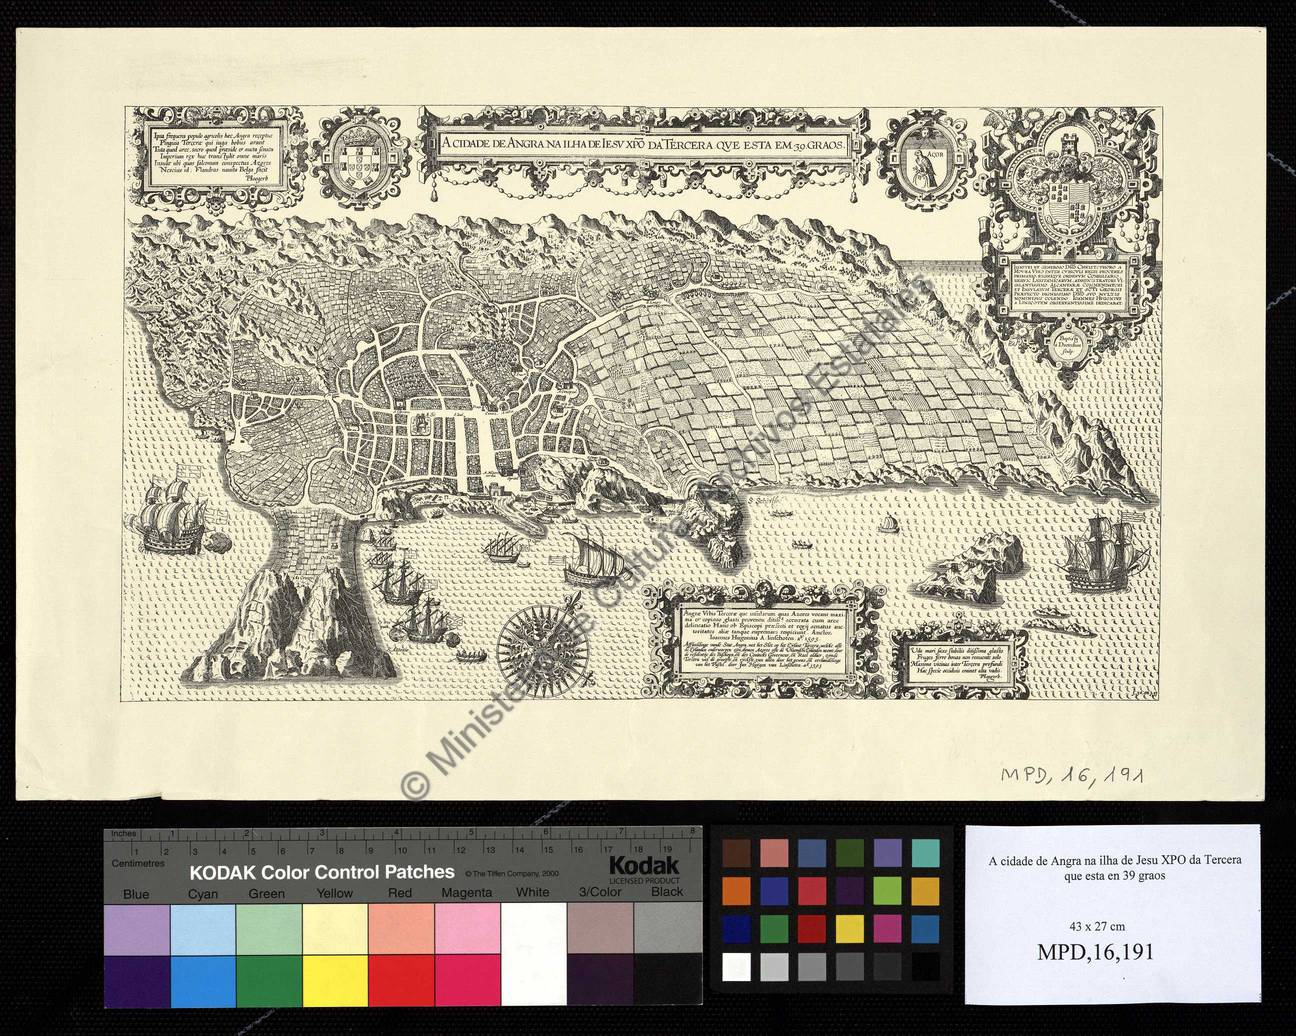
\includegraphics[width=\linewidth]{./images/map}
\caption{Digitized historical map}
\label{figure:map}
\end{figure*}

The digital revolution is affecting every part of our life. So the humanities scholars witness a change in their work life when analog collections are digitized. They have to apply algorithms to organize and analyze huge amount of data. The term ``digital humanities'' evolved during the last ten years and it can be defined as an intersection between the humanities and information technology  \cite{Svensson2010}. The information retrieval research group at the computer science department of the Universidad Nacional de Educación a Distancia (UNED) in Madrid cooperates with human scholars to conduct research in digital humanities. In their current project\footnote{\url{http://linhd.uned.es/p/proyecto-dimh}}, they work on historical maps. The maps have been drawn between 1503 and 1805, digitized and are available on the web\footnote{\url{http://www.mcu.es/ccbae/es/consulta/resultados_busqueda.cmd?busq_codsecc=MCAGS}}. These maps were annotated by human scholars. An example of a map is shown in Figure~\ref{figure:map} and its annotation are shown in Figure~\ref{figure:metadata}.\\

\begin{figure*}[!ht]
	\centering
	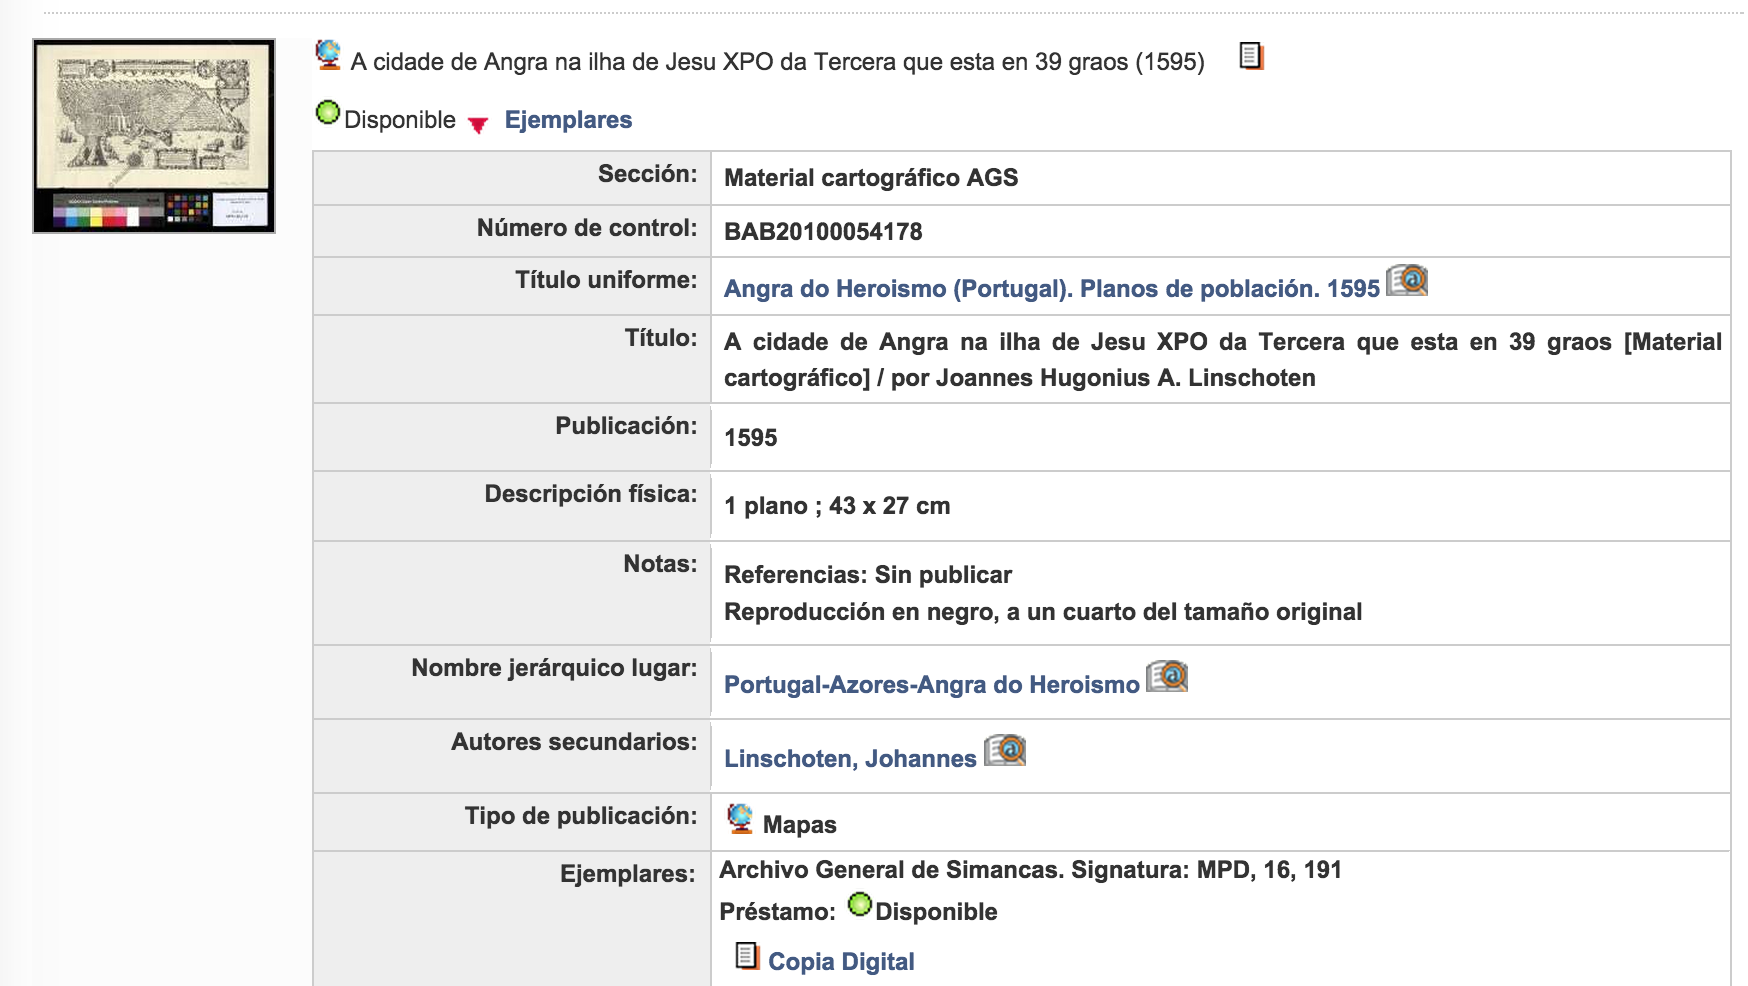
\includegraphics[width=\linewidth]{./images/metadata}
\caption{Annotation of a digitized map}
\label{figure:metadata}
\end{figure*}

To extract knowledge from the collection, the research group advocates \cite{Castellanos,Cigarran} for the use of a mathematical technique called Formal Concept Analysis \cite{Ganter2012}. After applying this technique, the maps are organized in a hierarchical structure which is called \textit{concept lattice}. A concept lattice is a special form of a \textit{lattice}. A lattice can be visualized statically in a \text{Hasse diagram}. An example of a Hasse diagram is shown in Figure~\ref{figure:hasse}. In this figure, you can see the power set of the set $\{x,y,z\}$ and the hierarchical relationships among them. The arrows indicate if a set (the origin) is a subset of another set (the destination). The nodes are layered in regard to the number of elements in a set. The node with all items is in the top and the empty set is in the bottom.\\

\begin{figure*}[!ht]
	\centering
	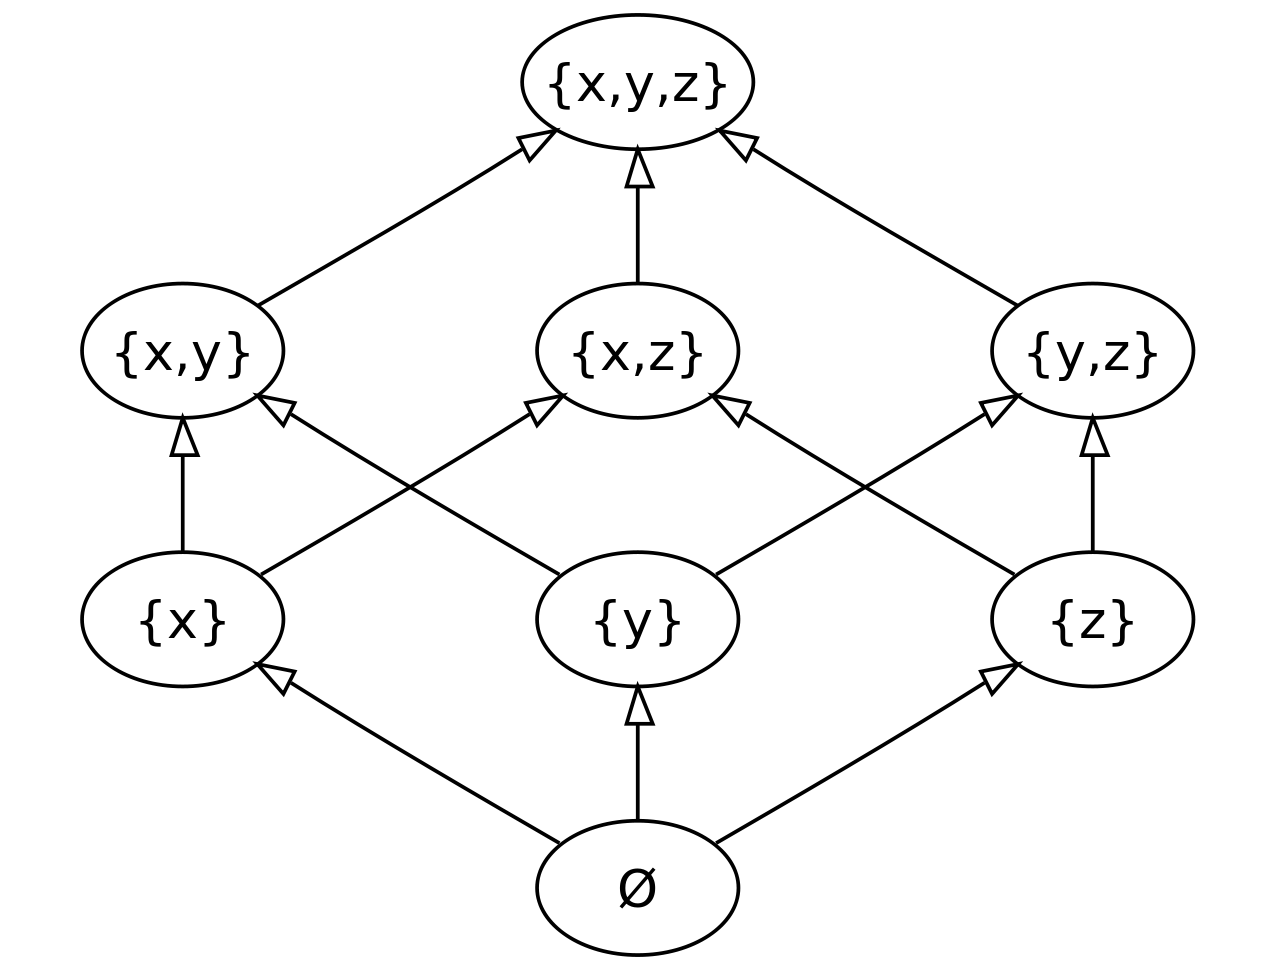
\includegraphics[width=\linewidth]{./images/hasse}
\caption{Hasse diagram, powerset of $\{x,y,z\}$ ordered by inclusion. Source: Anonymous Person \cite{hassediagramfig}}
\label{figure:hasse}
\end{figure*}

Because a concept lattice is also a lattice, concept lattices can be represented in Hasse diagrams. The research group successfully created a concept lattice of the maps and visualized it with a Hasse diagram. The result is shown in Figure~\ref{figure:firstVisualizaion}. They are not satisfied  with the visualization because it is nearly impossible to the see anything. The labels are overlapping, therefore it is hard to read them. It is not possible to distinguish between individual edges because of the huge amount of them. I did a twenty week internship at their research group and it was my task to create a useful visualization. \\

\begin{figure*}[!ht]
	\centering
	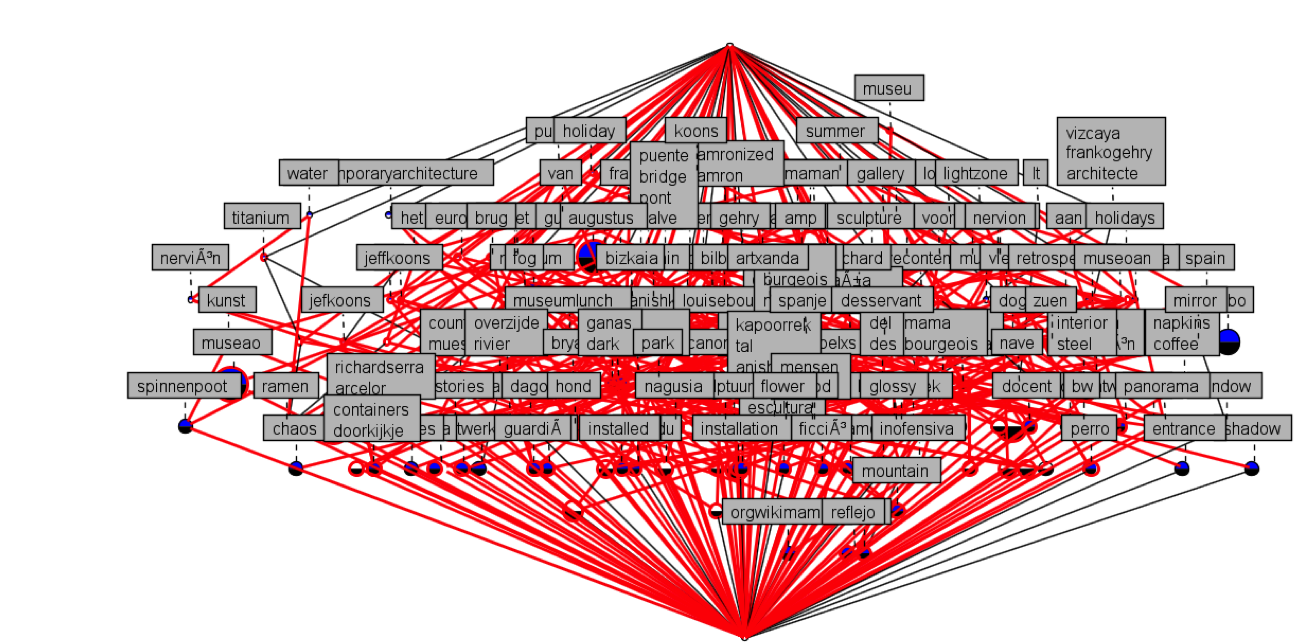
\includegraphics[width=\linewidth]{./images/firstVisualization}
\caption{First visualization of digital humanist data with traditional FCA software ConExp}
\label{figure:firstVisualizaion}
\end{figure*}

So the topic of this thesis is the theoretical elaboration about FCA and its visualization. This will lead to an own concept which will be implemented with the concept lattice derived from the collection of digitized maps. The implementation will be evaluated with a user study with five participants. The result of the study will show if my concept and its implementation are attractive for the users. It also possible to draw some conclusions about the given concept lattice (and FCA) itself, because the visualization can only be as good as its content.\\

 The remainder of this thesis is structured as follows: The background of Formal Concept Analysis and Interface Design Principles is presented in Section~\ref{Background}. The discussion of related work takes place in Section~\ref{Related Work}. Inferring from the related work, I will present my concept  and implementation in Section~\ref{Fancy 1.0}, which will  be evaluated in Section~\ref{Evaluation}. Built upon the conclusion of the evaluation, a new version of my work including a description about future words are presented in Section~\ref{Fancy 2.0}, before eventually concluding in Section~\ref{Conclusions}.
 
\chapter{Background}
\label{Background}

This sections provides background knowledge before we can discuss related work in the following section. Firstly, it gives an introduction into formal concept analysis taken from the work from Ganter and Wille \cite{Ganter2012}. Secondly, it introduces some basic interface design principles.

\section{Formal Concept Analysis}
\label{Formal Concept Analysis}

Formal Concept Analysis (FCA) is a mathematically well-founded technique to analyze data. FCA creates relationships among objects specified by attributes. It is derived from old philosophical ideas and was formalized by Rudolf Wille. In this section, I describe the formal background of FCA, its visualization, the use of FCA in information retrieval and eventually how FCA was applied to the digitized historical maps.

\subsection{Definition}

FCA \cite{Ganter2012} is constructed from a formal context. A \textit{formal context} is defined as a triple $K = (G, M, I)$ where $G$ is a set of objects\footnote{$G$ is derived from German \textit{Gegenstände}}, $M$ is a set of attributes\footnote{$M$ is derived from German \textit{Merkmale}} and $I$ is a binary relation $I \subseteq G \times M$. $I$ specifies whether an object has an attribute or not\footnote{$I$ is derived from German \textit{Inzidenzrelation}.}. Table~\ref{table:example} illustrates an example where $G$ comprises the integers from 1 to 10 and $M$ comprises the attributes composite, even, odd, prime and square. \\


\begin{table}[h]
\caption{Formal context, integers 1 to 10 as objects with attributes}
\label{table:example}
\centering

\def\arraystretch{1.2}% 
\begin{tabular}{ | c | c c c c c |}
\hline
  & composite & even & odd & prime & square\\
\hline

1 & & & $\times$ & &$\times$\\ 
2 & & $\times$ & & $\times$ &\\
3 & & & $\times$ & $\times$ &\\ 
4 & $\times$ & $\times$ & & & $\times$\\
5 & & & $\times$ & $\times$ &\\
6 & $\times$ & $\times$ & & &\\
7 & & & $\times$ & $\times$ &\\ 
8 & $\times$ & $\times$ & & &\\
9 & $\times$ & & $\times$ & & $\times$\\
10 & $\times$ & $\times$ & & &\\ \hline


\end{tabular}
\end{table}

Let the operator $'$ for $A \subseteq G$ be defined as following:
\begin{align*}
	A' = \{ m \subseteq M\; |\;  I(g, m)\;   \forall g \in A\}
\end{align*}

$A'$ is the set of those attributes that are present in all objects of $A$. \\

Let the operator $'$ for $B \subseteq M$ be defined as following:
\begin{align*}
	B' = \{ g \subseteq G\; |\;  I(g, m)\;   \forall m \in B\}
\end{align*}

$B'$ is the set of objects that have at least the attributes given in $B$. \\

$A$ is called \textit{closed}, if $A \subseteq G$ such that $A = A''$. The same is true for $B \subseteq M$ and $B = B''$. For example, let a set of objects be defined as $A_1 = \{1,4\} \subseteq G$. This results into: $A_1' = \{square\}$ and $A_1'' = \{1,4,9\}$. $A_1$ is not closed but $A_2 = \{1,4,9\} \subseteq G$ is called closed because $A_2 = A_2''$. \\   

A \textit{formal concept} is a pair of $(A, B)$ where $A \subseteq G$ and $B \subseteq M$ and $A = B' \wedge B = A' $. Informally, all objects in $A$ share exactly the same attributes in $B$. $A$ is a set of objects called the \textit{extent} of a formal concept. $B$ is a set of attributes called the \textit{intent} of a formal concept. The extent and the intent of all formal concepts are always closed. From the example in Table~\ref{table:example}, we can derive several formal concepts. Three randomly chosen concepts are shown in Table~\ref{table:exampleConcepts}. \\

\begin{table}[h]
\caption{Three formal concepts from the formal context in Table~\ref{table:example}}
\label{table:exampleConcepts}
\centering

\def\arraystretch{1.2}% 
\begin{tabular}{ c c c }
\hline
 Concept & Extent & Intent \\
\hline

$C_1$ & \{4,6,8,10\} & \{composite, even\} \\
$C_2$ & \{2,4,6,8,10\} & \{even\} \\
$C_3$ & \{9\} & \{composite, odd, square\} \\

\hline
\end{tabular}
\end{table}

It is always possible to define an order relation on the formal concepts. Let us introduce the relation $\le$ as follows:
\begin{align*} (A_i,B_i) \le (A_j, B_j) \Longleftrightarrow	A_i \subseteq A_j
\end{align*}

With the help of $\le$, we  can derive relationships from the concepts in Table~\ref{table:exampleConcepts}. We see that $C_1 \le C_2$. This means that $C_1$ is more specific than $C_2$ and $C_2$ is more general than $C_1$. We can also see that $C_3$ is unrelated to $C_1$, and that $C_3$ is unrelated to $C_2$. \\

A formal context with $\le$ is called a \textit{concept lattice} of the context. It can be shown that for two formal concepts $C_i$ and $C_j$, there always exists a formal concept $C_x$ such that $C_i \le C_x \wedge C_j \le C_x$. That means that there is always a formal concept wich is ``higher'' in the hierarchy and also related to the two formal concepts $C_i$ and $C_j$. A formal definition would exceed this section. The interested reader is advised to read "The Basic Theorem on Concept Lattices" as described by Carpineto and Romano on page 13 in their work \cite{carpineto2004concept}.\\

In the next section we will take a look at the static visualization of concept lattices.

\subsection{Static Visualization}

It is often said that a picture is worth a thousand words. To convey the information of a concept lattice, it can be visually represented in a \textit{Hasse diagram} \cite{Ganter2012}. Figure~\ref{figure:example} shows the Hasse diagram of the concept lattice derived from the formal context described in Table~\ref{table:example}. \\

\begin{figure*}[!ht]
	\centering
	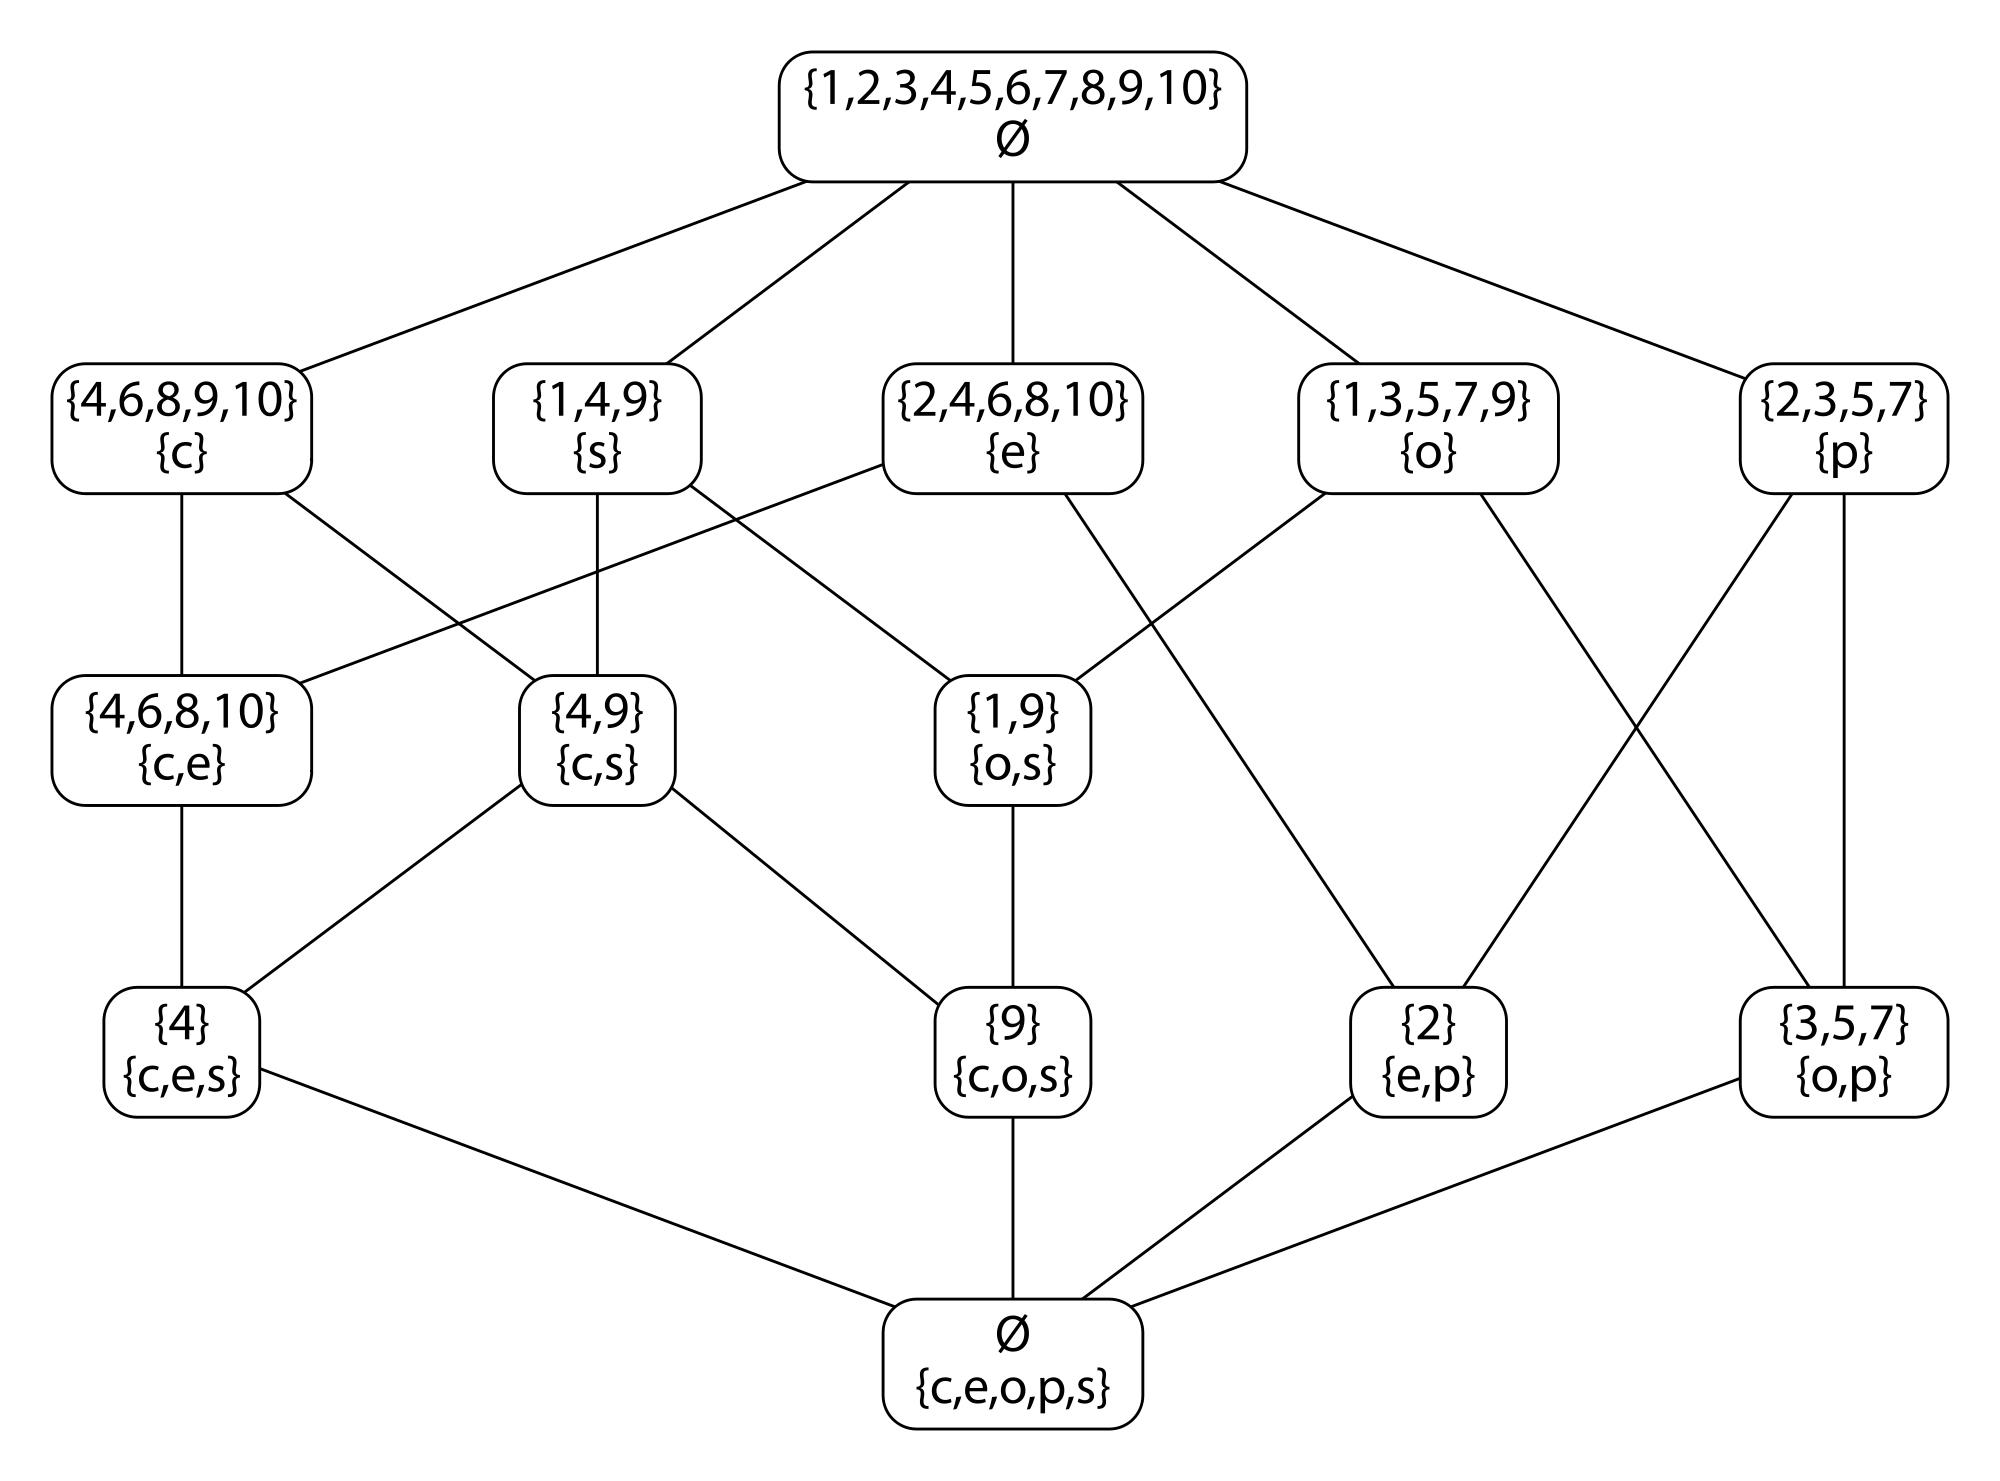
\includegraphics[width=\linewidth]{./images/fcaExample}
\caption{Hasse diagram, with the integers 1 to 10 as objects and attributes square (s), prime (p), composite (c), even (e), and odd (o). Source: Eppstein \cite{fcaexample}}
\label{figure:example}
\end{figure*}

A Hasse diagram is a graph where the vertices represent formal concepts and edges represent the relation $\le$ among the formal concepts. An edge between formal concepts $C_i$ and $C_j$ is drawn, when $C_i \le C_j$ and there does not exist a formal concept $C_x$ such as $C_i \le C_x \le C_j$. To increase the readability, the nodes are ordered in layers. The formal concepts at the top are more general, the formal concepts at the bottom are the more specific ones.\\

There are two special formal concepts: the \textit{supremum} and the \textit{infimum}. The supremum is the vertex in the top and the attributes in its intent are those which are present in all objects. In most cases its intent is empty, because it is rarely the case that an attribute is present in \textit{all} objects. The infimum is the vertex in the bottom and the objects in its extent are those which have all attributes. In most cases its extent is empty, because it is rarely the case that an attribute is absent in \textit{all} objects.\\

After this general introduction, I will describe in the next section how we can apply FCA to information retrieval. This is important because this thesis is based on a concept lattice that was created from a document collection.

\subsection{FCA and Information Retrieval}
\label{section:fcair}

Up to now, I only showed simple examples to illustrate the basics of FCA. So where was it applied? According to Poelmans et al. \cite{Poelmans2013}, FCA has been applied in many disciplines such as software engineering, knowledge discovery and information retrieval. They conducted two comprehensive surveys on the application of FCA \cite{Poelmans2013, Poelmans2013b}.\\

In the case of information retrieval, the objects are the documents. These documents are described by index terms, which are the attributes of the objects. The selection of appropriate index terms for a certain document is beyond the scope of this thesis. The interested reader finds more about this topic in the work from Manning et al. \cite{manning2008introduction}. Documents are described by index terms in Table~\ref{table:fcair} taken from Godin et al. \cite{Godin1993}. The concept lattice is visualized in Figure~\ref{figure:fcair}.

\begin{table}[h]
\caption{Documents described by Index Terms. Source: Godin et al. \cite{Godin1993}}
\label{table:fcair}
\centering

\def\arraystretch{1.2}% 
\begin{tabular}{ | l | l | }
\hline
 Document & Index Terms \\
\hline

1 & \{animal, bear, canada, child, cow-boy, dream, fantasy,\\
  & immigration, indian, magic\} \\
2 & \{animal, cat, child, fantasy, magic, tale\} \\
3 & \{animal, child, dog, fair, fantasy, love, parade\} \\
4 & \{child, fantasy, friendship, game, rope\} \\
5 & \{creativity, child, fantasy, game, music, sound\} \\
6 & \{animal, child, dream, fair, fantasy, friendship, octupus\} \\

\hline
\end{tabular}
\end{table}

\begin{figure*}[!ht]
	\centering
	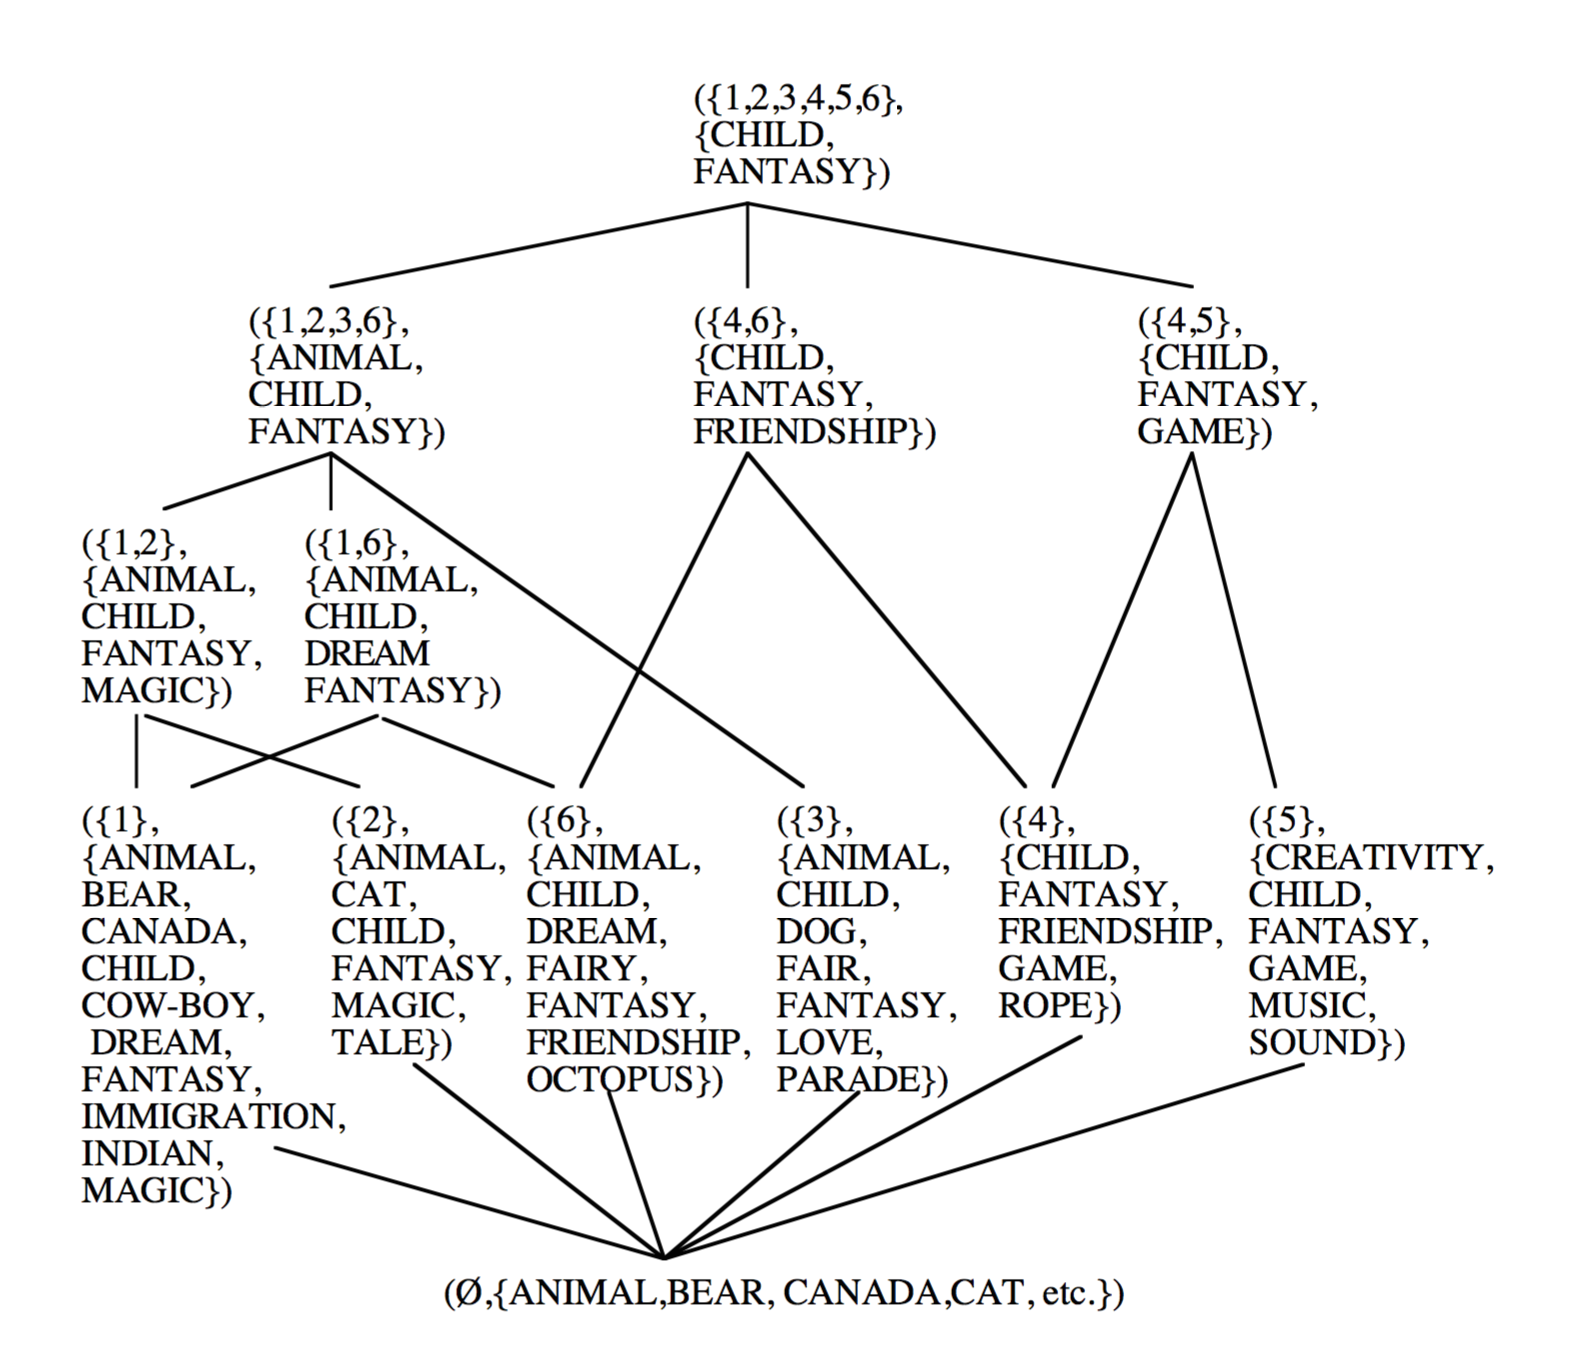
\includegraphics[width=\linewidth]{./images/fcair}
\caption{Hasse diagram from concept lattice derived from \ref{table:fcair}. One formal concept highlighted. Source: Godin et al. \cite{Godin1993}}
\label{figure:fcair}
\end{figure*}

Carpineto and Romano \cite{Carpineto2005} describe that a concept can be seen as a query (intent) with a set of retrieved documents (extent) and that neighboring concepts can be seen as minimal query changes. When the user queries a FCA-based system, the intents of the formal concepts are checked for a match (or a partial match if there is no match in the first place\footnote{It can happen that the query terms does not have a corresponding formal concept but a subset of other intents of formal concepts. This happens where there are other additional terms which always occur together with all terms of the query.}). So for instance with the query "child fantasy friendship" the documents 4 and 6 would be retrieved. You can find the formal concept surrounded with a circle in Figure~\ref{figure:fcair}.\\

Sacco and Tzitzikas \cite{Sacco2009} describe two information access modes: \textit{focalized search} and\textit{exploratory search}. In focalized search, the user is interested to find relevant information to a given query (which results from a known information need). In exploratory search, the user wants to explore the relationships among items in a data collection. While FCA provides the user with the ability to do focalized search, it also offers sophisticated exploratory capabilities. When the user queries the system (as described above), not only the documents of the formal concepts (which was determined based on the query) are retrieved, but she can also investigate the position of the corresponding node in the lattice. Is the node in the upper half and thereby more general? Or is it in the bottom half and thereby more specific? What are the related formal concepts? How do they differ? Would there be a lot more documents if I would remove a term from the query? All these questions can be answered and because the whole lattice is already computed, this can be done relatively fast. Without going into detail, a major problem of FCA is the time-consuming creation of a lattice. But the focus of this thesis is the visualization of concept lattices and not the creation of concept lattices. This section should give a slight introduction and the interested reader is advised to study the work from Carpineto and Romano \cite{carpineto2004concept} for a detailed investigation. \\

This thesis works with a given concept lattice to visualize it. Therefore it is important to understand how exactly it was created. The next section explains it.

\subsection{The Concept Lattice of the Digitized Maps}
\label{thedata}

The research group built the concept lattices based on the annotations of 7492 maps. The first step is to construct the index terms of the documents. For this, they asked some human scholars for terms that they are interested in. They collected 100 terms which are the possible index terms. A document is described by an index terms if it occurs in the documents at least once. For this, the different dimensions of the annotations like author, location etc. are treated as a single document without any separation between the dimensions. From these index terms, they built the concept lattice which contains 131379 formal concepts.\\

Because this thesis focuses on the user interface, let us review user interface design principles before we discuss related work in Section~\ref{Related Work}.

\section{Interface Design}
\label{id}

The user interface is responsible for the interaction with users. The interaction of humans with computers has its own research area, Human-Computer Interaction (HCI), and one of its pioneers is Ben Shneiderman. In the following, two of his principles will be presented: The "Eight Golden Rules of Interface Design" \cite{Shneiderman2010} and the "Visual Information Seeking Mantra" \cite{Shneiderman1996}.

\subsection{Eight Golden Rules of Interface Design}
\label{Golden}

These rules \cite{Shneiderman2010} are general advices for user interface designers which should apply to all interfaces. The rules are named and explained with my own remarks. \\

\begin{itemize}
	\item Strive for consistency: Use similar actions in similar situations. Use identical terminology, colors, fonts etc. throughout the system.	
	\item Cater to universal usability: Design for the needs of a diverse user group (skill level, age, gender or other differnces)
	\item Offer informative feedback: Give system feedback for every action.
	\item Design dialogs to yield closure: Sequences of actions should be grouped. Give feedback on completion of a group.
	\item Prevent errors: Design the system so that the user cannot even do errors in the first place. But if she does some, offer instructions how to recover.
	\item Permit easy reversal of actions: Actions should be undoable. This gives the user confidence to explore the system.
	\item Support internal locus of control: The user should think that she is in charge.
	\item Reduce short-term memory load: Reduce the number of things the user has to keep in mind while using the system.
\end{itemize}

There exist alternative principles, for instance: Donald Norman's Design Principles \cite{Norman2013} or Jakob Nielsen's "10 Usability Heuristics for User Interface Design" \cite{Nielsen1995}. They are very similar and only differ in insignificant details.\\

These principles can be applied to all user interfaces. In the next section, design principles will be presented which are more related to this work.

\subsection{Visual Information Seeking Mantra}

The visual information seeking mantra (the Mantra) was introduced by Ben Shneiderman \cite{Shneiderman1996} and is based on his experience with past projects. Albeit the Mantra was intended to be a "descriptive and explanatory" \cite{Card1999} one, "in effect, the Mantra has become a prescriptive principle for many information visualization designers”, write Craft and Cairns \cite{Craft2005}. \\

The Mantra describes design principles for interfaces when users view collection of items. These items are described by multiple attributes. The starting principles are: overview first, zoom and filter, and then details on demand. These four principles will be explained below and extended by three other principles.
\begin{itemize}
	\item Overview: Gain an overview of the entire collection.
	\item Zoom: Zoom in on items of interest.
	\item Filter: Filter out uninteresting items.
	\item Details-on-demand: Select an item or group and get details when needed.
	\item Relate: View relationships among items.
	\item History: Keep a history of actions to support undo, replay, and progressive refinement.
	\item Extract: Allow extraction of sub-collections and of the query parameters.
\end{itemize}

Some tasks need more explanation.

\subsubsection{Zoom and Filter}

These tasks are responsible for reducing the complexity of the data collection. 'Zoom' means that the user focuses on items she wants to see. 'Filter' means that she can hide items which are not interesting for her.

\subsubsection{History}

It is important to give the user the possibility to easily recover from mistakes or loss of interest. In addition, "it is rare that a single user action produces the desired outcome. Information exploration is inherently a process with many steps, so keeping the history of actions and allowing users to retrace their steps is important”, writes Shneiderman \cite{Shneiderman1996}.

\subsubsection{Extract}

Once interesting objects are found, the user should have the possibility to extract them from the system. Shneiderman describes printing, emailing or saving the item to the disk as 'extraction'.

\subsection{Final Remarks}

The presented ideas are based mostly on the experience of one person: Ben Shneiderman. The huge number of citations show that his work is influential but Craft and Cairns \cite{Craft2005} call for empirical justification of the Mantra. HCI is a young research area, better and more polished guidelines will emerge the future. Until then, the work from Ben Shneiderman seems to be a valid starting point. \\

These principles are up to interpretation and adaption. Every system is different and has its different needs. For this reason, let us review what other people did and how they designed their interface for FCA-based systems.

\chapter{Related Work}
\label{Related Work}

After introducing formal concept analysis in Section~\ref{Formal Concept Analysis}, let us review and discuss related work. In the first three sections, I go over different FCA-based approaches. Eventually, we evaluate one FCA-based approach in detail: The Virtual Museum of the Pacific. In Section~\ref{dyafs}, a non-FCA based approach is shown which is related to FCA: Faceted Search. \\

\section{Full Hasse Diagrams}

The traditional static visualization of concept lattices are Hasse diagrams as described in Section~\ref{Formal Concept Analysis}. Eklund et al. \cite{Eklund2004} conducted user studies and proclaim that non-FCA-experts can read Hasse Diagrams if you fine-tune the Hasse diagram. For instance by choosing appropriate colors, using symbols and carefully positioning the vertices in layer. \\

But in the domain of information retrieval you get formal contexts with a lot of objects. Hasse diagrams scale badly for large concepts lattices. Kuznetsov et al. \cite{Kuznetsov20072}  describe this resulting visualization: "Representing concept lattices constructed from large contexts often results in heavy, complex diagrams that can be impractical to handle and, eventually, to make sense of." Especially the high connectivity of the graph results in enormous edge crossing. The Figure~\ref{figure:firstVisualizaion} shown in Section~\ref{Introduction} shows the first result of the research group. The visualization is useless because it is not even possible to see all the labels. In the next section I describe techniques to improve the situation.

\section{Pruned Hasse Diagrams}

The Hasse diagrams can be pruned by reducing the number of vertices. The different techniques are discussed in the next section.

\subsection{Reduce Number of Formal Concepts}

One way to reduce the number of vertices is to compute the \textit{iceberg lattices} as described by Stumme et al. \cite{Stumme2002}. They result from the application of a data mining technique "frequent item-set mining" from Agrawal et al. \cite{Agrawal1993}. Only formal concepts are selected which are considered "frequent". A formal concept is frequent if its intent, the set of attributes, is frequent. Let $B$ be the intent and $minSupport \in [0, 1]$, then $B$ is frequent if $ |B'|/|G| \geq minSupport$. This means the attribute set has to specify a high portion of objects; at least $minSupport$. This approach has some drawback as Kuznetsov et al. \cite{Kuznetsov20072} point out that "exotic" or "emergent" concepts that are not represented by a large number of objects can be interesting too and should not be overlooked. They propose to only select "stable" concepts \cite{Kuznetsov20072}. The intent of stable concepts does not depend much on each object of the extent. It is also possible to apply traditional cluster techniques like fuzzy K-Means clustering to FCA \cite{AswaniKumar2010}. \\

	While all these techniques undoubtably reduce the number of formal concepts, it is to question whether the results are of any help. In our case of information retrieval, we apply FCA to explore the data and get insights about the lattice structure. When pruning the nodes, you are losing many data relationships, many formal concepts and, consequently, the "power" of FCA as exploratory technique is significantly reduced. When we deal with large concept lattices, the number of nodes has to be very low if we want to represent them with Hasse diagrams. Nowadays, the question is not how do I visualize 16 formal concepts as in Figure~\ref{figure:example} - it is rather how can I visualize 160000 formal concepts.\\
	
	Pruning alone is not a proper way to handle large concept lattices. But it can be useful in combination with techniques that are presented in Section~\ref{Local View} to reduce the clutter.
\subsection{Nest Formal Concepts}	

Another approach is the use of \textit{nested line diagrams} - line diagrams are another name for Hasse diagrams. For this, all attributes are partitioned into layers. For example, if you just have two layers, an attribute is either in layer one or two. For the first layer: You built up a Hasse diagram with the attributes \textit{solely} of the first layer. For each vertex in the resulting Hasse diagram, you built up a Hasse diagrams \textit{inside} the vertex. These secondary Hasse diagrams are built from the concept lattice derived from the objects in the vertex (the objects that are the extent of the formal concept). This can be done for an arbitrary number of layers. An example from Carpineto and Romano \cite{carpineto2004concept} is shown in Figure~\ref{figure:nested}. The general idea should be clear without explaining the context - if not, Carpineto and Romano \cite{carpineto2004concept} describe it in more detail. \\

\begin{figure*}[!ht]
	\centering
	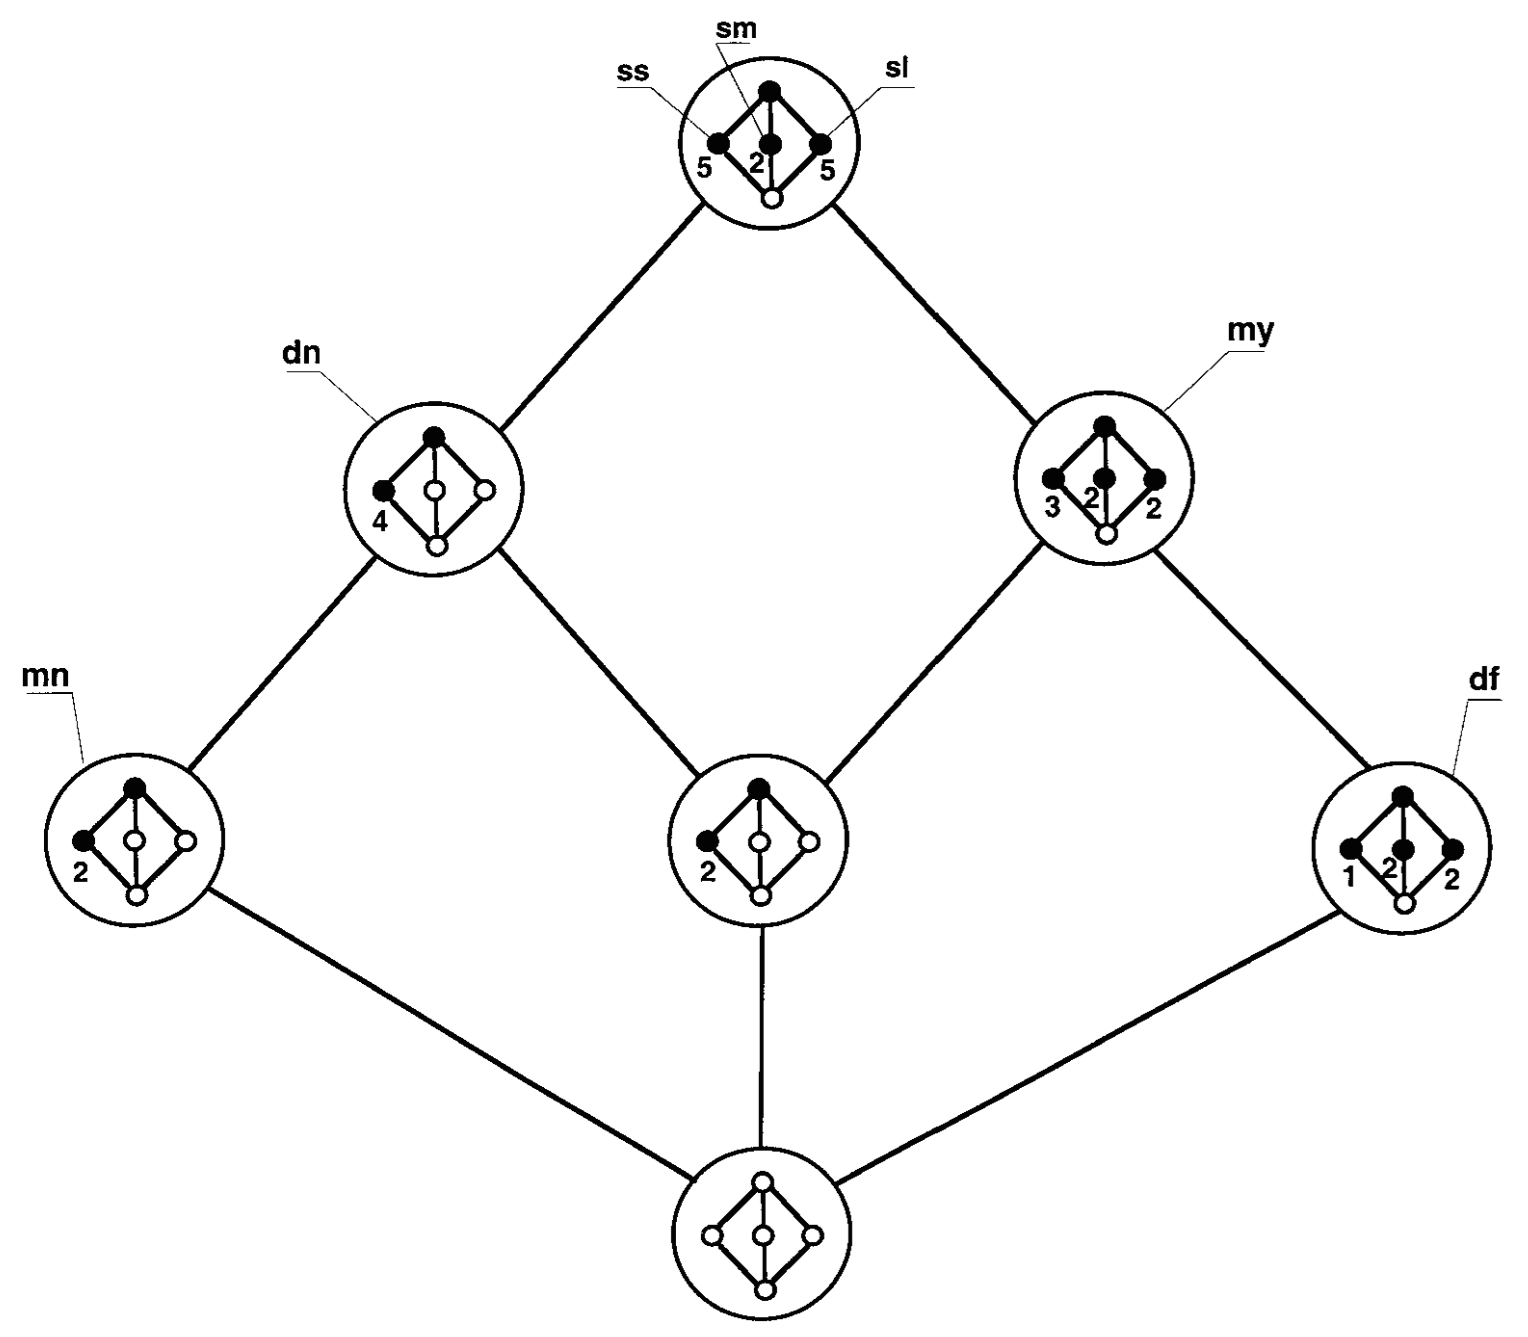
\includegraphics[width=\linewidth]{./images/nested}
\caption{Nested Hasse diagram with two layers. Source: Carpineto and Romano \cite{carpineto2004concept}}
\label{figure:nested}
\end{figure*}
	
But how to partition the attributes? You have to select the partitions manually. The manual selection might be a good idea for small concept lattices but in our case, it is not feasible.

\section{Local View}
\label{Local View}

Instead of showing the full Hasse diagram, the user can have a local view on the lattice. I will give an overview about the basic idea and applications before we review one real-world application in detail.

\subsection{Basics}

One could argue that you just have to visualize everything and then allow to zoom on nodes. This techniques is common among network visualizations \cite{Herman2000}. But because of the high connectivity of the graph, this is not helpful to Hasse diagrams. You can see this in the tool ``FCART'' presented by Neznanov and Parinov \cite{Neznanov2014}. In Figure~\ref{figure:fcart} they visualize a concept lattice comprising more than 20000 concepts. \\

\begin{figure*}[!ht]
	\centering
	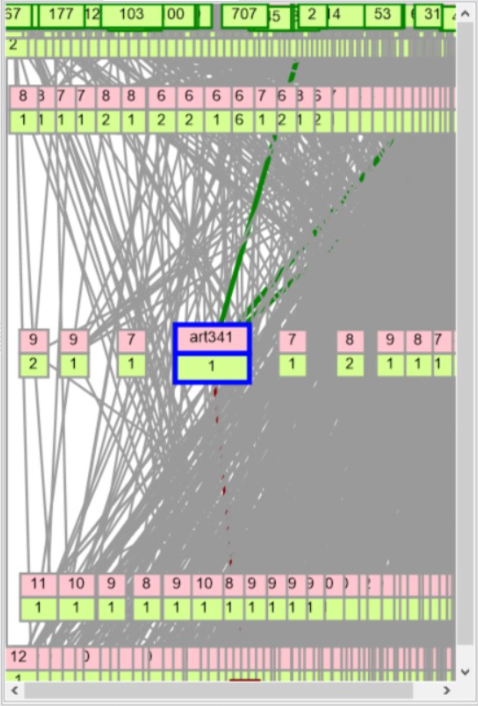
\includegraphics[width=0.5\linewidth]{./images/fcart}
\caption{FCART, Hasse diagram with over 20000 formal concepts, focus on node with blue borders. Source: Neznanov and Parinov \cite{Neznanov2014}}
\label{figure:fcart}
\end{figure*}

Even though they chose a light color for the edges, the screen is almost filled only with the the color of the eges. In addition, the labels of the nodes in the top and bottom are overlapping which makes it hard to read them. Let us review some other approaches in the next section which completely break with the Hasse diagram. \\

The local view on a Hasse diagram is called \textit{conceptual neighborhood} by Eklund et al. \cite{Eklund2009,Eklund2012}, \textit{hybrid navigation} by Carpineto and Romano \cite{Carpineto1996} or \textit{semantic probe} by \cite{crampes2014visualizing} by Crampes and Planié. The basic idea is always the same: The interface is always focused on exactly \textit{one} formal concept. The user can navigate through the lattice by going up (becoming more general) or going down (becoming more special), which means removing terms or adding terms. They also offer the possibility to query the system. In most cases, the user would start with a search and focus on the corresponding formal concept if it exists. From there, the user can fine-tune the search. The idea originated from the information retrieval field and was first proposed by Godin et al. \cite{Godin1989}. \\

At least three ideas underly this approach. Firstly, users tend to start with a short query and then refine their needs. Hearst \cite{Hearst2009} writes while referring to \cite{Marchionini2006,Bates1990}:
\begin{quote}
	A commonly-observed search strategy is one in which the information seeker issues a quick, imprecise query in the hopes of getting into approximately the right part of the information space, and then doing a series of local navigation operations to get closer to the information of interest.
\end{quote}

Secondly, it is easier for the users to choose from suggestions than to formulate a query. Aula \cite{Aula2005} writes that searching is a more demanding method for locating information than browsing, as it involves several phases, such as planning and executing queries, evaluating the results, and refining the queries, whereas browsing only requires the user to recognize promising-looking links. \\

Third, after the initial search, the neighboring concepts are basically suggestions to the users. This prevents them from getting empty results. This is related to the design principle: "Prevent errors" presented in Section~\ref{Golden}. Zero results are not really errors, but they can be seen as a failure in a search process.\\

Godin et al. \cite{Godin1993} evaluated their FCA-based approach in comparison to boolean retrieval and hierarchical retrieval and proclaim that their experiment suggests that retrieval using a concept lattice may be an attractive alternative since it combines a good performance for subject searching along with browsing potential.

\subsection{Applications}
Carpineto and Romano picked up the idea from Godin et al. and developed a FCA search engine ULYSSES \cite{Carpineto1995,Carpineto1996}. The user can fine-tune what neighboring vertices are displayed by bounding the information seeking space. They are not only showing directly adjacent vertices but also vertices that do not exceed a given distance. It is also possible to restrict the space to vertices which are above, below, left or right of the focus. The system is shown in Figure~\ref{figure:ulysses}. \\

\begin{figure*}[!ht]
	\centering
	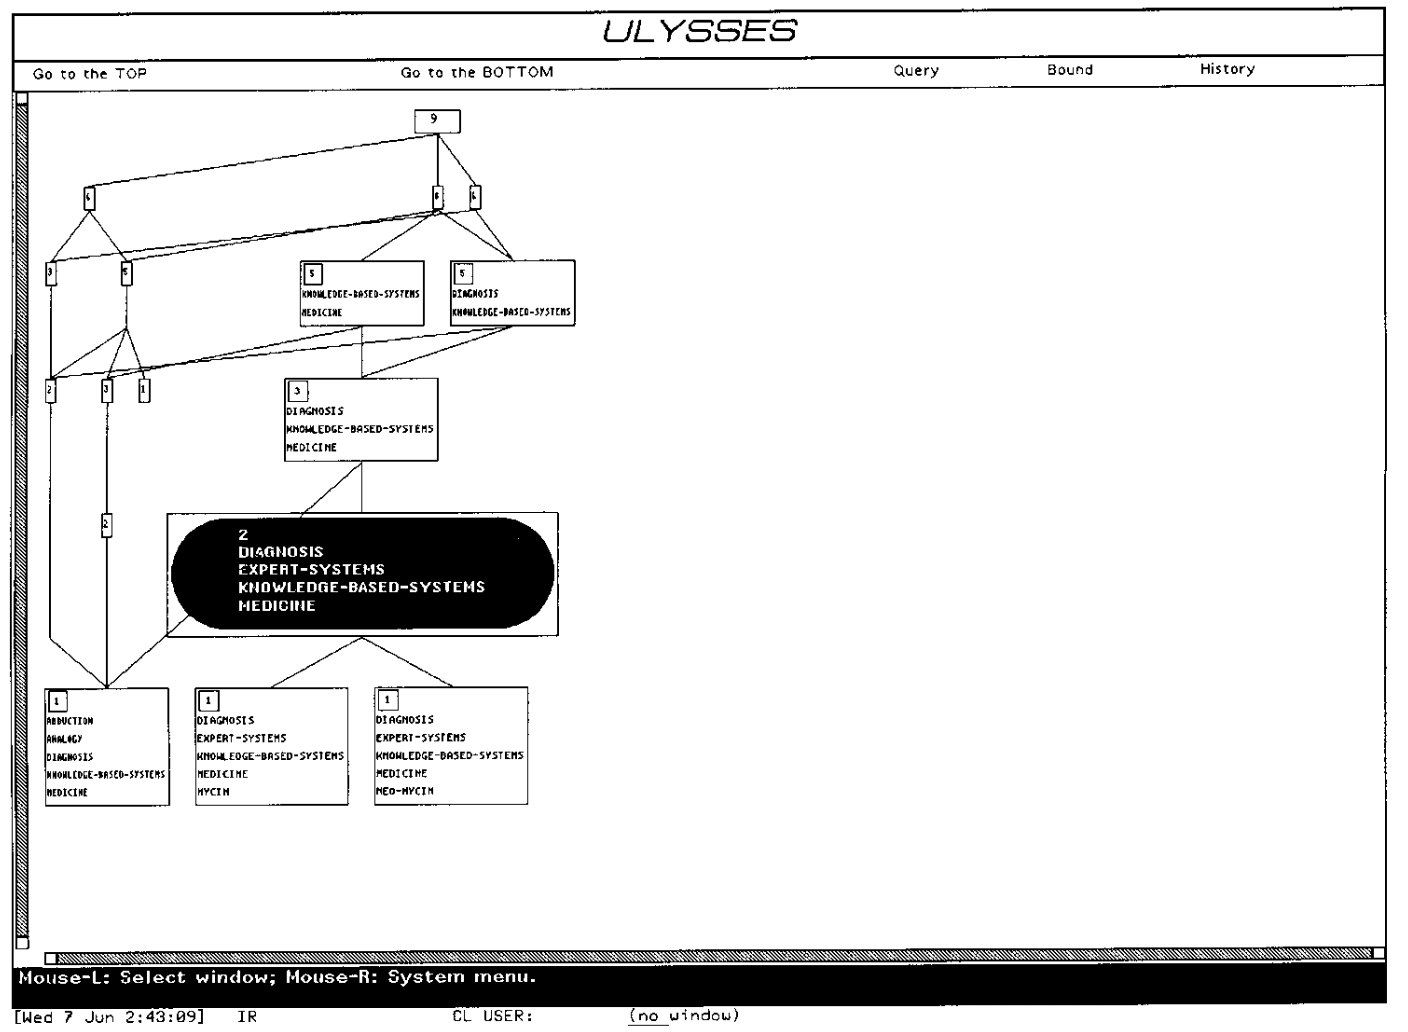
\includegraphics[width=\linewidth]{images/ulysses}
\caption{ULYSSES with focus on the black node. Source: Bach \cite{Bach2010} }
\label{figure:ulysses}
\end{figure*}

\begin{figure*}[!ht]
	\centering
	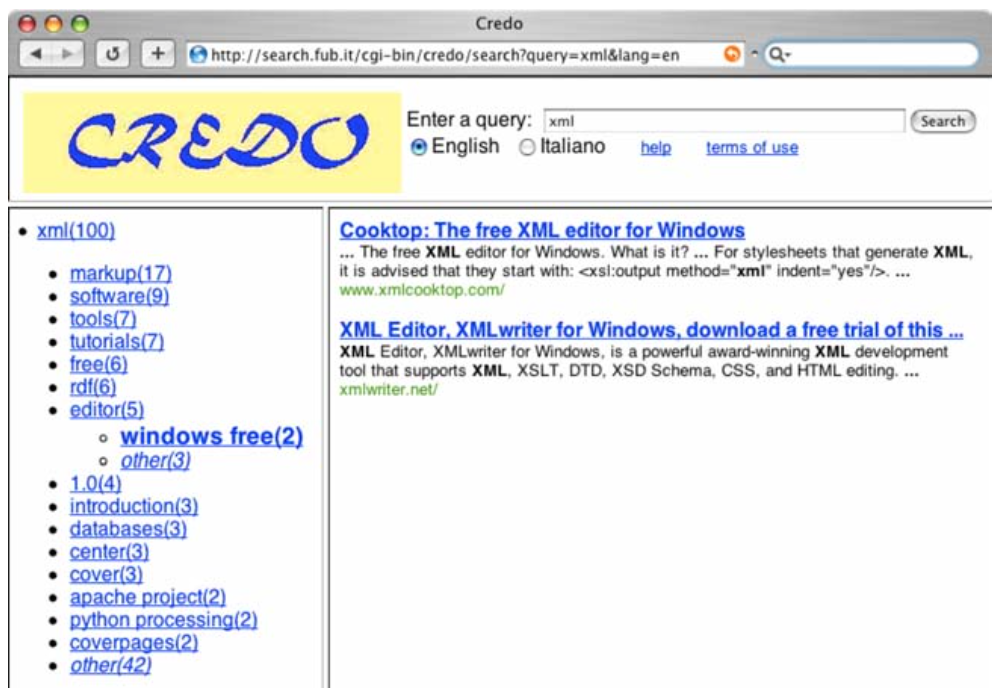
\includegraphics[width=\linewidth]{images/credo}
\caption{CREDO, after query ``xml'' and browsing after ``editor(5)'' and ``windows free(2)''. Source: Carpineto and Romano \cite{Carpineto2004} }
\label{figure:credo}
\end{figure*}

In their work, CREDO \cite{Carpineto2004}, Carpineto and Romano followed the look of ordinary search engines. The presentation of the concept lattice is not oriented at the Hasse Diagram. It looks more like a folder structure. It is shown in \ref{figure:credo}. Work that is similar comes from Koester \cite{Koester2006}, Dau et al. \cite{Dau2008}, Nauer and Yannik \cite{Nauer2009} and Cigarran et al. \cite{Cigarran2004}. In all these cases, FCA is applied in slightly different manner. The search is done with ordinary search engines in the background (e.g. Yahoo!) and the concept lattice is built from the results of the search. So for every new search, there is a new concept lattice. This is different from our approach, where there is just one static concept lattice. \\

Let us now review work of FCA on document collections. Eklund et al. applied FCA to email organization \cite{Eklund2004}, image browsing \cite{Ducrou2006,Ducrou2008} and a later work is the ``Virtual Museum of the Pacific'' \cite{Eklund2009,Eklund2012}. I will focus on the museum because it does exactly what we are trying to do: Visualize a concept lattice built from image metadata. Furthermore, it is a rare example of FCA outside of the academic community. It also runs in the browser and it was built in 2009 - so it is fairly recent. In addition, they conducted a usability study with museum experts and non-experts \cite{Eklund2012}.

\subsection{Virtual Museum of the Pacific}
\label{Museum}
 
The museum was created to give users the possibility to browse images of museum objects. It is available on the web\footnote{\url{http://epoc.cs.uow.edu.au/vmp/} - Credentials are required. Use username: filter and password: 45755} and it is advised to take a look at it before continue reading. \\

\begin{figure*}[!ht]
	\centering
	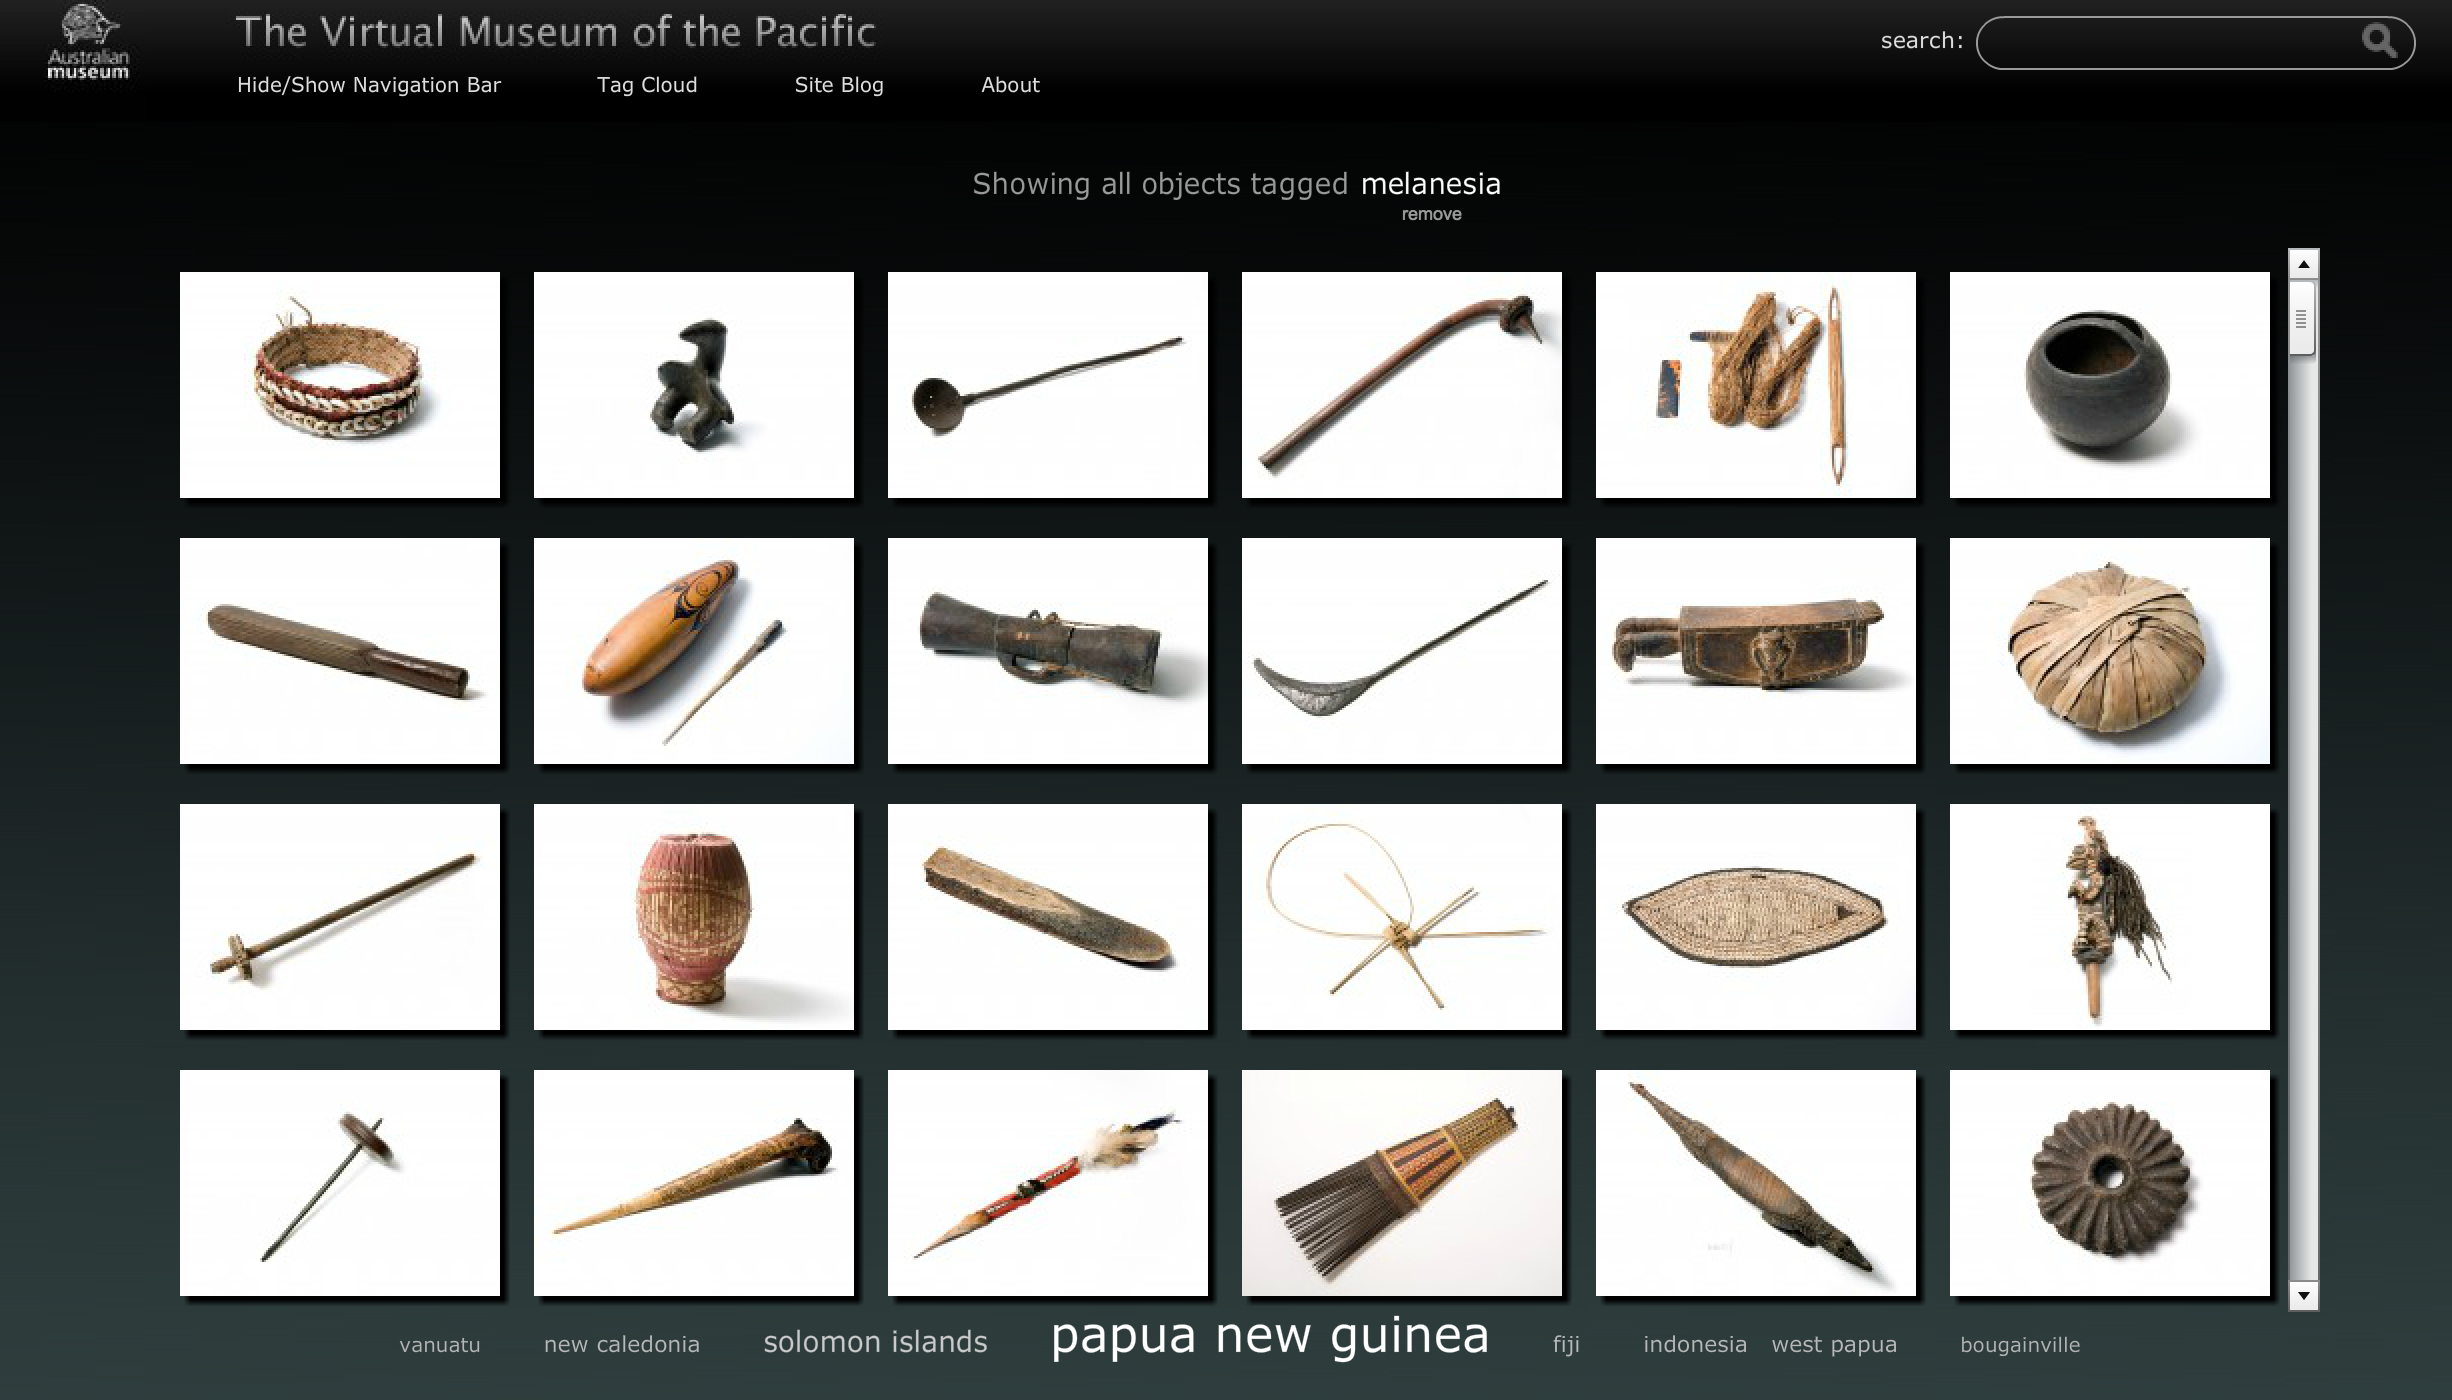
\includegraphics[width=\linewidth]{images/pacific}
\caption{The Virtual Museum of the Pacific, focus on concept ``melanesia''}
\label{figure:pacific}
\end{figure*}

After the login, the user can either search on the collection or get an overview over the collection by clicking "tag cloud" or "browse perspective". The interface sets the objects, the images, in the focus of the interface. This is, in my opinion, a good decision. The user is probably more interested in the objects than in the concept lattice. The lattice is just an artificial structure that was built around the objects. \\
 
The intent of the focused formal concept is above the objects. It is possible to remove terms from the current selection to generalize (go up in the lattice). Below the objects are terms suggested to specify the information needs (go down in the lattice). The view changes when the users decide to add or remove terms. The sidebar categorizes the attributes into topics. It looks like they have created a taxonomy for their attributes. This allows the users to filter out interesting terms.\footnote{But the manual creation of a taxonomy is time-consuming. It is also to question if FCA should be applied to datasets with a taxonomy. If you have a taxonomy of your data, this means that your data comprises of several dimensions. In this case, you can user other techniques. The Section~\ref{dyafs} will describe one of those techniques.} If you click on an item, you can investigate the details of the item. From there you can also find related items.\\
 
It is possible to search but this search is very basic because it does not offer any term suggestions or other help. The designers of the virtual museum should have stuck to well-proven user search interface principles as described by Hearst \cite{Hearst2009}. The biggest problem is the missing "home" or "reset" button and the absence of any form of history. As Shneiderman \cite{Shneiderman1996} points out, "Information exploration is inherently a process with many steps, so keeping the history of actions and allowing users to retrace their steps is important." We saw in Section~\ref{section:fcair} that FCA can bee seen as an exploratory technique. Not implementing \textit{any} possibility to backtrack is a huge problem. You can see in the evaluation that users were confused. Eklund et al. write \cite{Eklund2012}:
 \begin{quote}
 Users also had difficulty understanding the notion of conceptual navigation as a way of navigating an information space, rather than a fixed hierarchy with a well defined `home' state. [..] Many users felt `lost' within [the FCA-based] style of navigation. A recommendation was put forward so that users could at least back track through the navigation sequences (in the form of a `Back' button) or that users could easily go back to a `home' or `reset' state.
 \end{quote}
  In my opinion, they are not addressing these problems - even though the navigation is a big part of the interface. It feels like that they are blaming the problems on the unfamiliarity of the users when they write \cite{Eklund2012}: "there were a number of common issues [with the interface], mostly relating to the unfamiliarity of the interface". This is a weak argument because users are always unfamiliar with new interfaces. But after all, this evaluation gave valuable insight into the perception of users with a local view navigation.
  
\subsection{Conclusion}

The Virtual Museum of the Pacific is one of the few examples of FCA that breaches traditional static visualizations. They idea to show only the directly related formal concepts is promising because this scales better than Hasse diagrams. My concept is based upon the work from the museum but addresses critical problems: the missing orientation, the missing history and the basic search interface. The concept is described in Section~\ref{Fancy 1.0}. Before that, let us review a related non-FCA-based technique.

\section{Faceted Search}
\label{dyafs}

This section should only give a small overview about this technique. Completely introducing it is beyond the scope of the thesis. Additional information can be found in the work from Sacco and Tzitzikas \cite{Sacco2009}. To keep things short, this technique is explained with an example. Figure~\ref{figure:flamenco} shows a screenshot of Flamenco as described by Yee et al. \cite{Yee2003}. \\

\begin{figure*}[!ht]
	\centering
	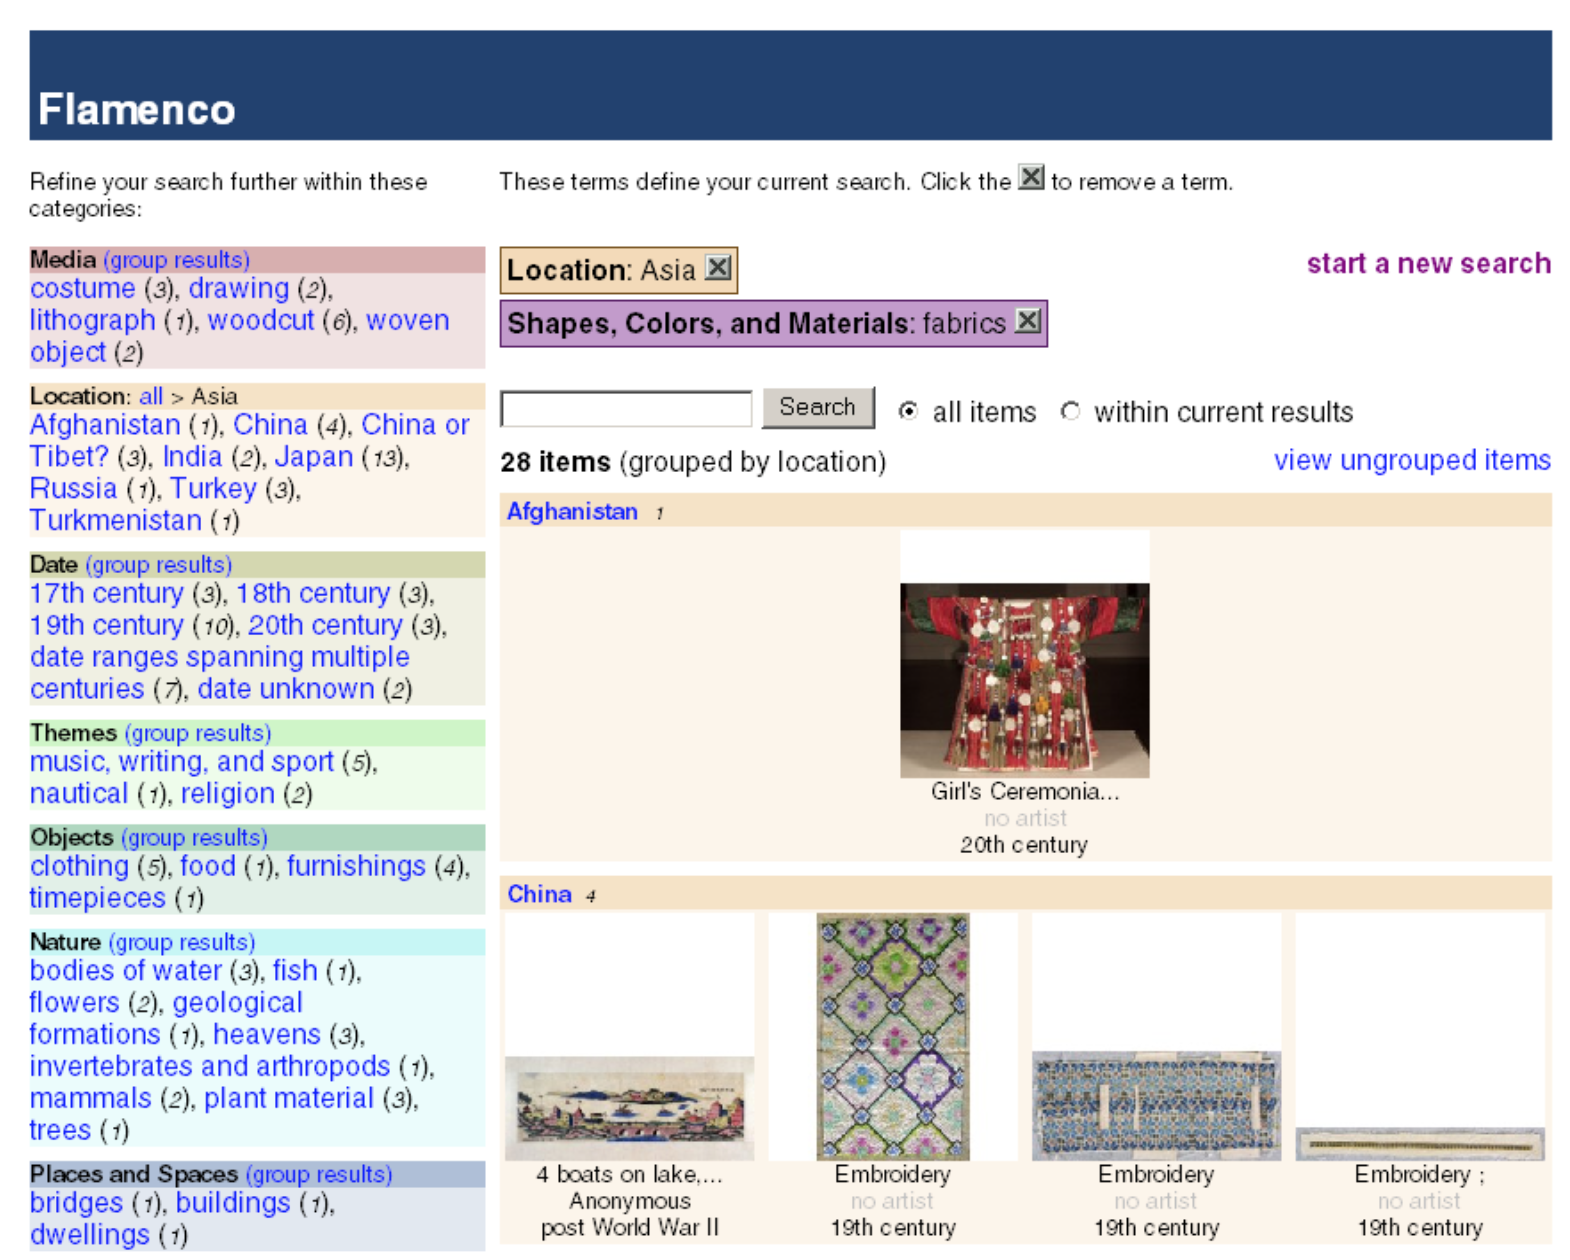
\includegraphics[width=\linewidth]{images/flamenco}
\caption{Flamenco, only items that are from Asia and made from fabrics are shown. Source: Yee et al. \cite{Yee2003}}
\label{figure:flamenco}
\end{figure*}

This interface is similar to the "local view" on Hasse diagrams presented in Section~\ref{Local View}. The main idea: The dataset comprises several dimensions called \textit{facets}. The user can restrict dimension to certain values. Only items which fulfill the restrictions given by the user are shown. In addition, the user gets suggestions for further restrictions. In Figure~\ref{figure:flamenco}, you can see that the location is restricted to "Asia" and shapes etc. are restricted to "fabrics". On the left, you can see the suggestions and how many items would be left after restricting. \\

Sacco and Tzitzikas \cite{Sacco2009} say that although FCA and Faceted Search are apparently two distinct approaches to information modeling and access, and they use a different terminology, they are closely related. They also mention that faceted search reduces the cognitive efforts because it ensures that the results are manageable. It feels like faceted search is superior to the local view on concepts lattice, if the data consist of more than one dimension. For this reason, the use of FCA for this particular dataset is questionable because it actually comprises several dimensions (author, location, time et al.). Nevertheless, the research group applied FCA and it was my task to visualize the concept lattice. The resulting interface is described in the next section.

\chapter{Fancy FCA 1.0}
\label{Fancy 1.0}

First, a concept is described to visualize large concept lattices. Second, this concept is implemented as an interactive web application. The data (in form of a concept lattice) for this implementation comes from the research group as it was described in Section~\ref{thedata}. Third, the concept and the implementation are discussed.

\section{Concept}

The concept of the interface is inferred from discussing the related work in Section~\ref{Related Work}. It is influenced mainly by the Virtual Museum of the Pacific discussed in Section~\ref{Museum}. They follow the idea to only give a local view on the Hasse diagram. This is done because the concept lattices of most formal contexts are too large to visualize them in a Hasse diagram. In this form, the interface always focuses on one formal concept called \textit{the Focus}. Only directly related children of the Focus are shown. The initial state of the Focus lies on the supremum. The supremum is the most general formal concept. The user has two possibilities to change the Focus:
\begin{enumerate}
	\item She can select a child of the Focus as new Focus.
	\item She can ``jump'' to a completely new Focus by using a search on the lattice\footnote{It is very important to realize that the search is NOT done on the documents. It is only done on the attributes of the objects of the formal context. Informally, the search is only done on the index terms of the documents. If the users search for terms that are not the index terms of any documents, it will result in an error.}
\end{enumerate}
Let me demonstrate this with an example shown in Figure~\ref{figure:conceptExample}. After searching on the lattice after the attribute ``e'', the Focus is set to the formal concept surrounded with a dashed circle. Now, only the nodes surrounded with a black circle are visible to the user. These two formal concepts are called \textit{the Suggestions}, because they suggest the users which attributes to add to the current selection of the Focus. In this case, there is one suggestion to add ``c'' to the focus and refine the selection from 5 objects (2,4,6,8,10) to 4 objects (4,6,8,10). And the suggestion to add ``p'' to the focus and refine the selection to one object (2). They are the children of the Focus and therefore by definition more specific than the Focus. \\

\begin{figure*}[!ht]
	\centering
	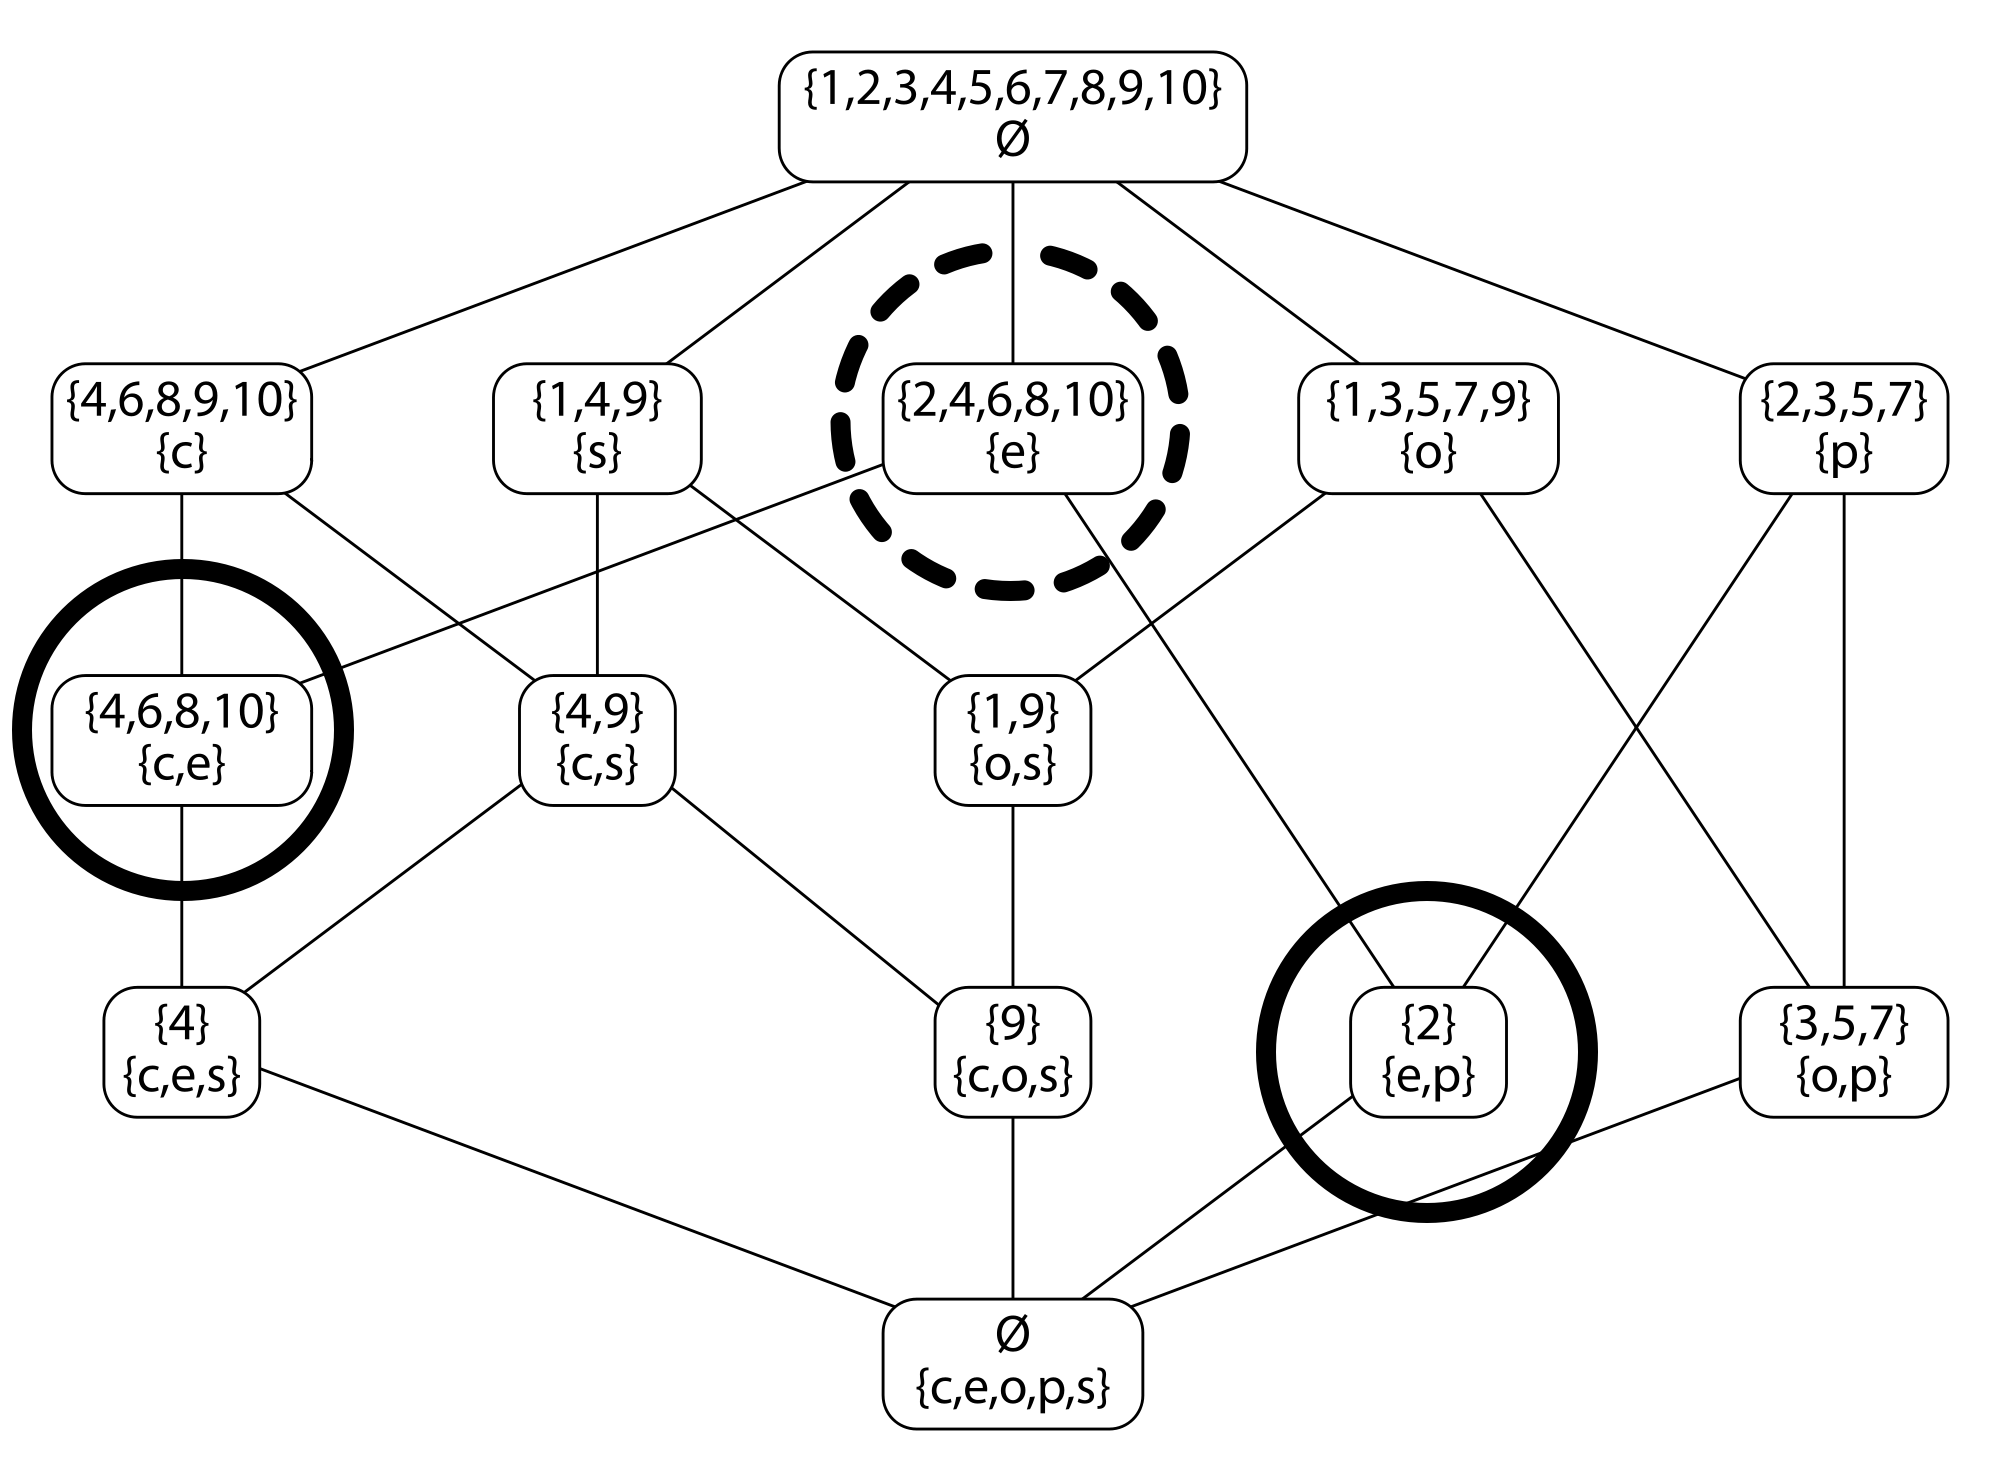
\includegraphics[width=\linewidth]{images/focus}
\caption{After searching for ``e'' the Focus lies on the formal concept with a dashed circle. Only its children (black circles) are visible to the user. }
\label{figure:conceptExample}
\end{figure*}

We discussed the problems of the Museum earlier and realized that the users need some additional orientation with this kind of local view. Therefore we give them two possibilities to do so:
\begin{itemize}
	\item \textit{Breadcrumbs}: The breadcrumbs show the trail how the user got to the current Focus. The term comes from Hänsel and Gretel fairy tale\footnote{\url{https://en.wikipedia.org/wiki/Hansel_and_Gretel}}. It is often used in web pages to give orientation. They typically look like ``Home / Selection1 / Selection2''.
	\item \textit{History}: Offer an overview about the history of the navigation actions.
\end{itemize}

Let me describes these actions in detail after taking a look at the genreal interface layout.

\subsection{Interface Components}
After describing the general navigation, we can already identify two important components of the interface: A \textit{Search Bar} and the \textit{Suggestions}. The users are probably also interested in the \textit{Results}. The Results are those objects from the Focus. Also the \textit{Breadcrumbs} and the \textit{History} are components to be shown. The components of the interface are completed with a \textit{Menu} and you can see the general layout in Figure~\ref{figure:schema}. The components are described in detail now. \\

\begin{figure*}[!ht]
	\centering
	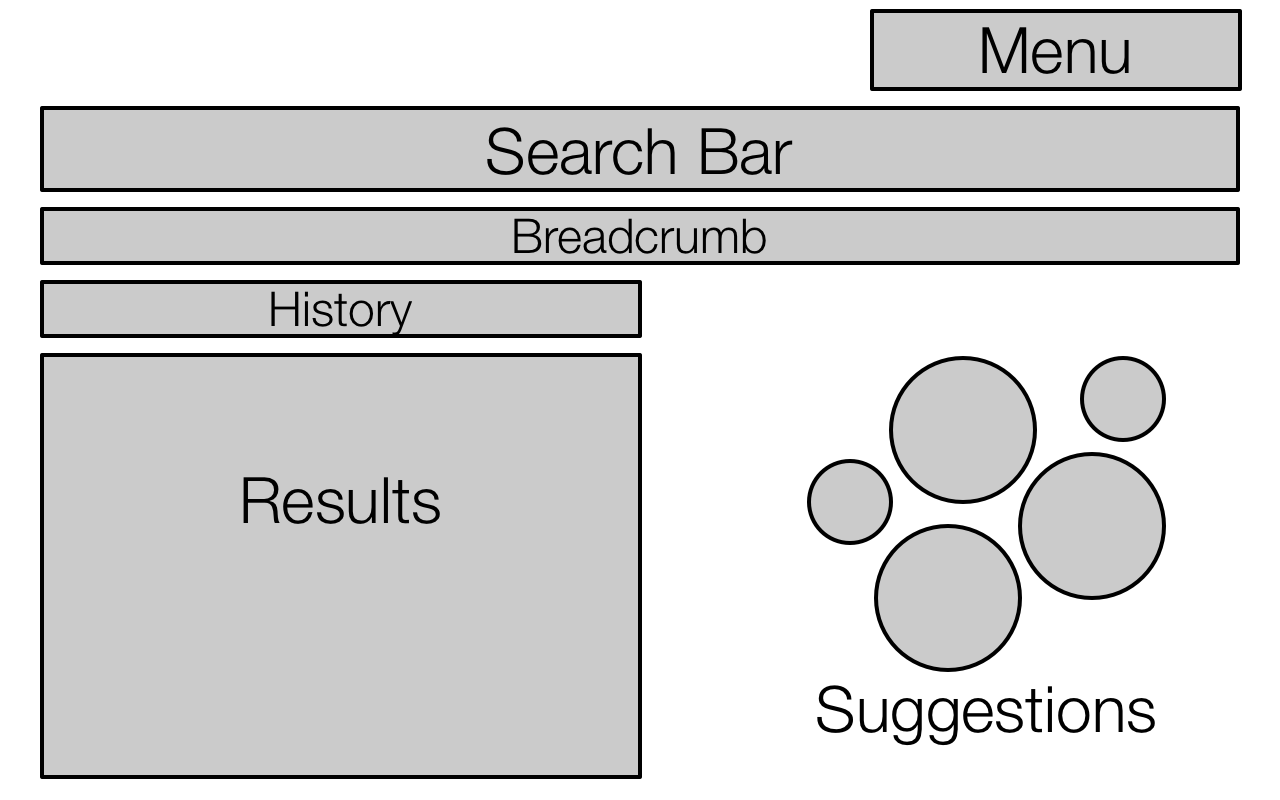
\includegraphics[width=\linewidth]{images/schema}
\caption{Wireframe of the interface of Fancy FCA 1.0}
\label{figure:schema}
\end{figure*}

\subsubsection{Search Bar and Results}

All users know web search engines. In my opinion, it is easy for users to work with a new system if it looks similar to systems they already know. That is why the overall look of the interface should remind users of search engines. The general advices to design user search interfaces by Hearst \cite{Hearst2009} should be followed. Results should be ordered in a vertical list. Each list item consists of a title and a snippet. The title describes the items in short and the snippet goes more into detail. They can review the result in detail by clicking on the title. The title links to a web page where the user can investigate the results in detail. The snippet should give the users a small overview about the results. In addition, the user should have the possibility to bookmark the result if she is logged in. This was done because of Shneiderman's recommendation to let the user extract results.

\subsubsection{Suggestions}

The different suggestions are shown as a bubble cloud. Each bubble stands for one formal concepts and it is only labelled with terms that should be added. The size of the bubble corresponds to the number of documents the formal concept has. The exact number is shown as tooltip when the user hovers over the bubble.

\subsubsection{Breadcrumbs}

Breadcrumbs are included to give the user orientation. The Breadcrumbs indicate how the user got to the current focus. Of a given Focus, it shows the parental formal concepts of the Focus. It is really hard to describe it abstractly. So let us have a look at an example. The user starts with the initial Focus. From there he searched for ``x''. Then he clicked on the suggestion ``y''. The breadcrumbs show ``Home / x / y''. The current Focus has the terms ``x y''. Each part of the breadcrumbs links back the previous focus. If you click on ``x'', the Focus changes back to the Focus with ``x''. If you click on ``Home'', you end up in the initial Focus. This should increase the orientation of the user because the user always knows how she can get to the start and she knows her current selection. It also increases the confidence of the user to just try out clicking a suggestion. If she does not like it, she can always go back easily. 

\subsubsection{History}

With the history, the user can look back his navigational history. It exceeds the possibility of the Breadcrumbs to backtrack because the Breadcrumbs can only show a few steps back. When the user ``jumps'' to a completely new Focus, the Breadcrumbs cannot help her to go back to previous Focuses. With this History, she can go back to all previous focuses. If the user is logged into the system, the all-time history is collected and shown. If not, only the history of the current \gls{session} is shown. If the users starts using the site and logs in after some time, all the previously collected \gls{session} history should be send to the server as well. The history is basically a list of history items. A history item is described by the terms of the Focus. In the proposed wireframe, the History panel is small, because it is collapsed (hidden) to the user most of the time. When the panel is clicked, it will uncollapse and show all the history items. This was done to save space.\\

All together, an UML use case diagram can be drawn which is shown in Figure~\ref{figure:usecase}. You can see that the user needs to authenticate to the system (login) to use some functionalities.

\begin{figure*}[!ht]
	\centering
	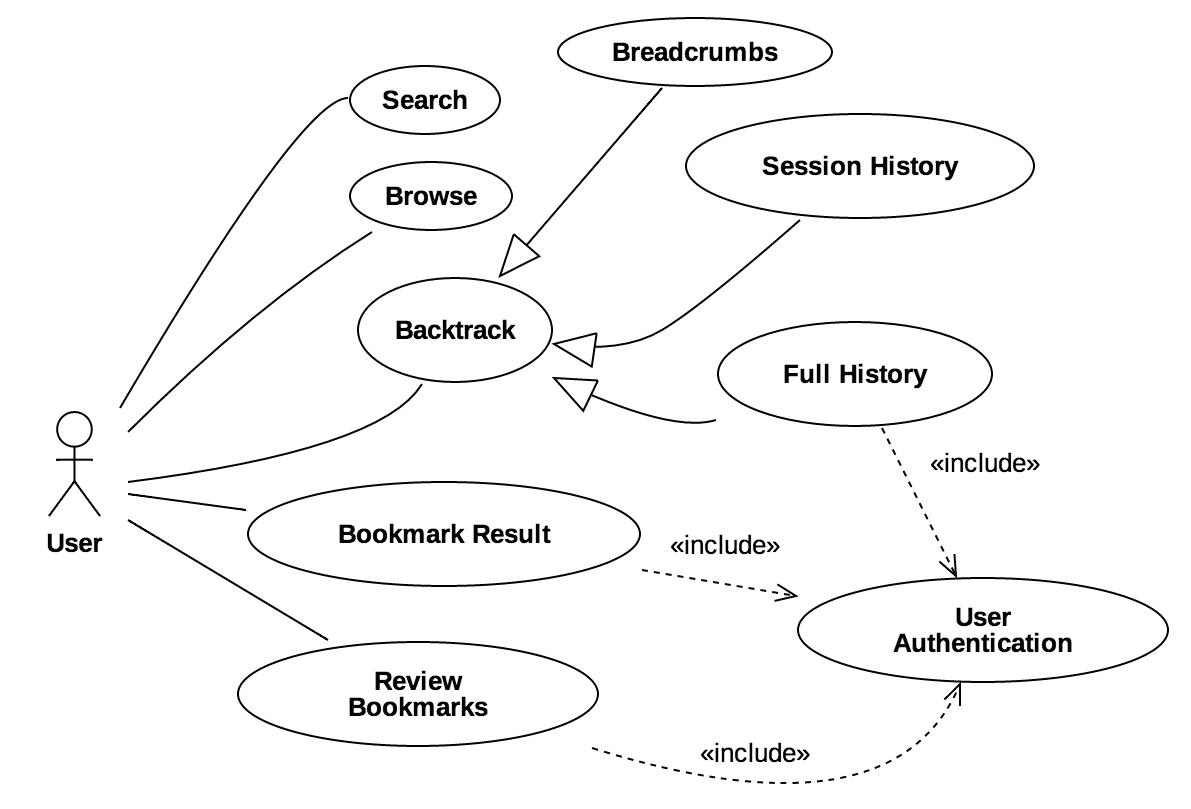
\includegraphics[width=\linewidth]{images/usecase}
\caption{UML use case diagram for Fancy FCA 1.0}
\label{figure:usecase}
\end{figure*}

\section{Implementation}

The implementation was done with data provided from the research group. So they gave the already computed lattice and all the information of the documents. You can find the system running at \url{http://fancy.vis.one} and a 30-seconds video of it here. \\

The implementation is done as a web application because all users already have a web browser installed. There is no setup necessary. The implementation of a web application can be split up into client side  and server side part. The server side is responsible for the programming code that runs on the server and for the databases. The client is responsible for the code that runs in the browser and all the visual elements the user can interact with. Let us start with the server side.

\subsection{Server Side}

It has to be decided first, which programming language and framework to use for the web application. I chose Express.JS \footnote{\url{http://expressjs.com}} of the runtime environment Node.JS\footnote{\url{https://nodejs.org}} because it uses the programming language JavaScript. JavaScript is also used for the client side because it is the only programming language which runs in a browser. So we only need to stick to one programming language if we use JavaScript. But instead of writing JavaScript, we use CoffeeScript\footnote{\url{http://coffeescript.org}}, which adds \gls{syntactic sugar} to JavaScript and compiles to JavaScript.\\

We need a database to store data. The research group wanted to store logs\footnote{The logs were never evaluated because the tool was never used in production.} of the user interaction. In addition, we have to save the history of users and their bookmarked documents on the server. For this, I use MySQL as database because it was already installed on the server where the software should run. Because of the use of an object-relational mapping (ORM) framework, Sequelize \footnote{\url{http://sequelizejs.com}}, the database can be changed easily. The ORM creates an abstraction and it allows the programmer to interact with the database without writing raw SQL queries.

\subsection{Client Side}

Because the interface is a webpage, the used technologies were HTML, CSS and JavaScript. HTML is the markup language to create webpages and the backbone of the web. CSS adds style to the webpages. JavaScript adds interactivity to the webpages. But like on the server side, instead of writing pure JavaScript I programmed in CoffeeScript which was compiled into JavaScript. I used the framework Bootstrap\footnote{\url{http://getbootstrap.com}} because it allows me to quickly create appealing webpages. Bootstrap has templates for all kinds of components like forms, buttons, navigational elements, a grid system, icons etc.. Instead of reinventing the wheel, I use Bootstrap to use basic components.\\

Now let us take a look at some screenshots of the system to demonstrate the implementation. In Figure~\ref{figure:fancy1}, you can see the initial state of the interface. The bubble cloud on the right shows the Suggestions. It is a little bit unorganized but the initial state has to show the most Suggestions. This is because this state is the most general formal concept. Most of the time, the bubble cloud is more organized because there are less Suggestions. For the layout of the bubbles, I use the JavaScript framework D3\footnote{\url{http://d3js.org}} \cite{Bostock2011}. D3 utilized SVG to draw elements which are also accessible via the Document Object Model (DOM) API, which means I can catch events like ``mouse over an item'' or ``click on an item''. The bubble cloud is a customized graph force-directed layout based on the work from Vallandingham \cite{Vallandingham}. \\

\begin{figure*}[!ht]
	\centering
	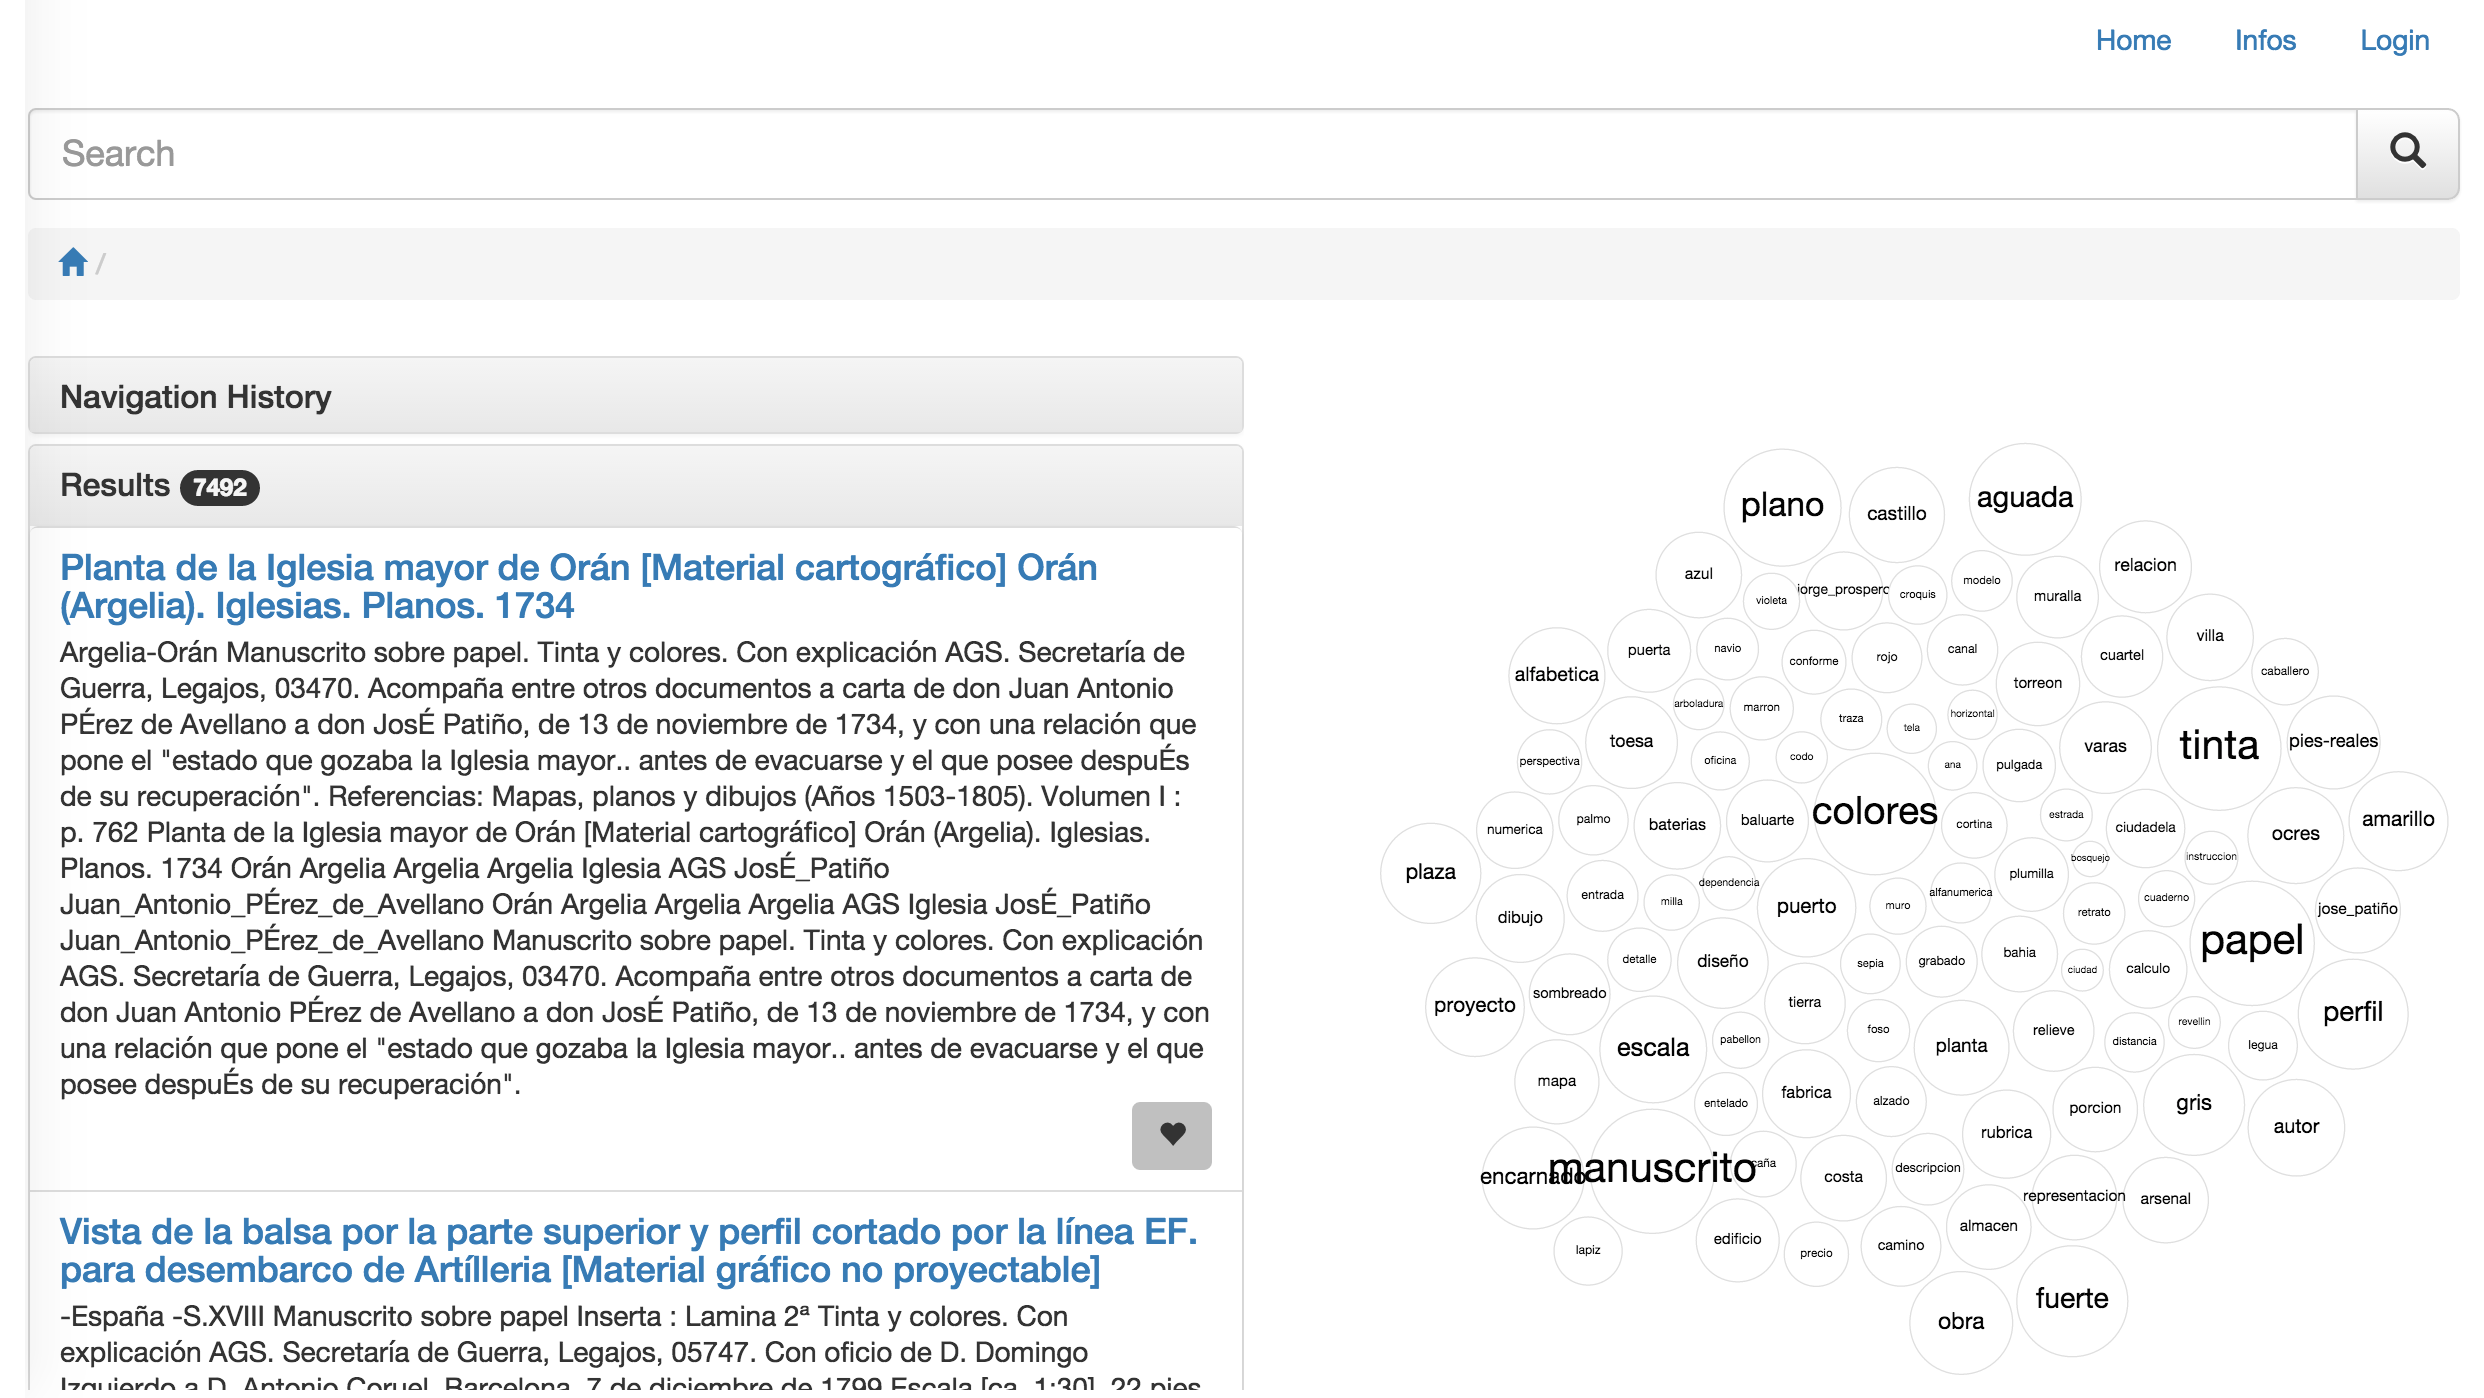
\includegraphics[width=\linewidth]{images/fancy1}
\caption{Fancy FCA 1.0, initial state}
\label{figure:fancy1}
\end{figure*}

 In Figure~\ref{figure:fancy2}, you can see the use of a ``Typeahead'' which can also be called ``auto-complete''. For this, I use the JavaScript library Twitter typeahead.JS\footnote{\url{https://twitter.github.io/typeahead.js}}. In Figure~\ref{figure:fancy3}, you can see two screenshots which both focus on the left part of the interface. Let us start with the left one. In there, we can see various components. Starting with the search bar, we can see the terms of the Focus. We are looking for documents with the index terms ``papel tinta fabrica''. Below the search bar, you can see the breadcrumbs. They allow, for instance, to backtrack to just the Focus ``papel tinta'', if the user clicks on ``tinta''. Below the breadcrumbs, you can see the label ``Navigational History''. But first, let us take a look at the ``Results''. The number after ``Results'' show how many results there are, in this case 227. Let us take a look how the result items are presented. First, there is a title. If you click on the title, you will get to an external webpage with further information. Below the title is a snippet of the result. The terms of the Focus are highlighted. In the bottom right corner, you see the icon to bookmark this item. Now imagine to click on the ``Navigational History'' label. Then, the interface changes into the picture on the right in Figure~\ref{figure:fancy3}. There, you can see that the ``Navigational History'' is uncollapsed. It shows a list of History items. If you click on an item, the Focus changes. \\
 
\begin{figure*}[!ht]
	\centering
	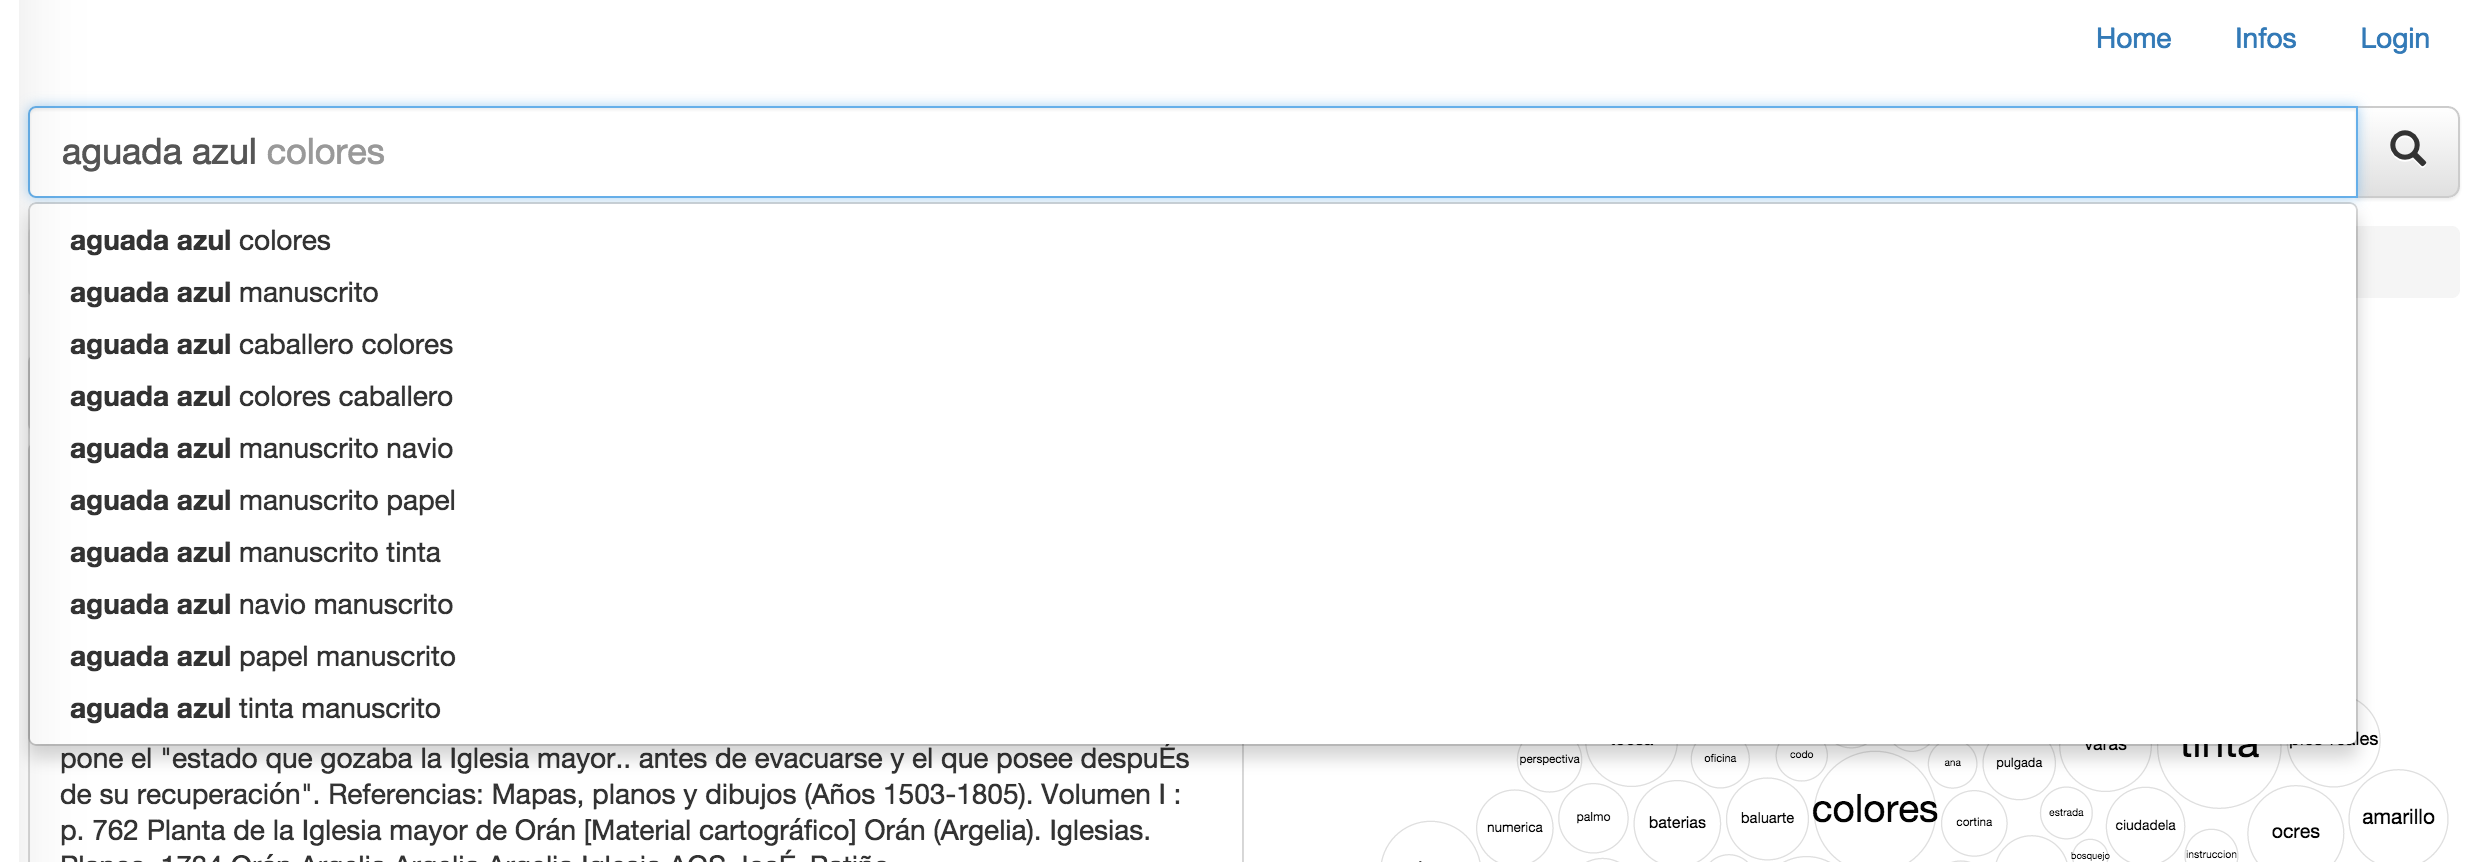
\includegraphics[width=\linewidth]{images/fancy2}
\caption{Fancy FCA 1.0, search interface offering Typeahead}
\label{figure:fancy2}
\end{figure*}

\begin{figure}[!ht]
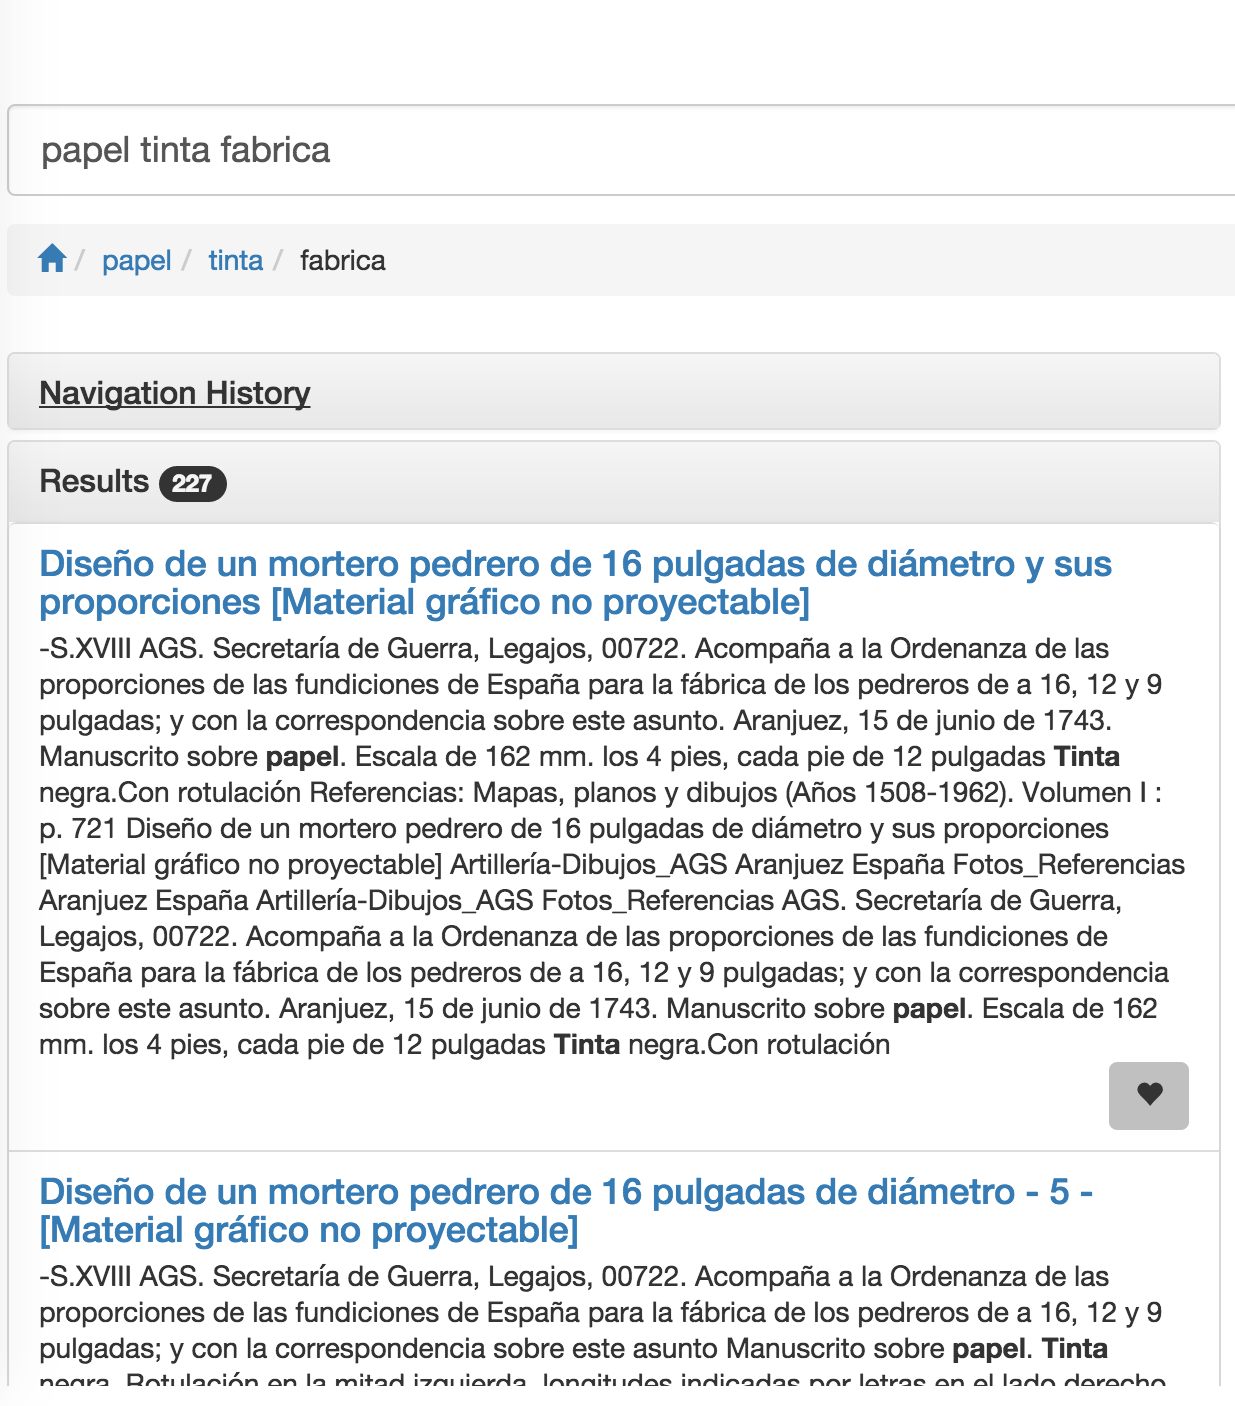
\includegraphics[width=.48\linewidth]{images/fancy4}\hfill
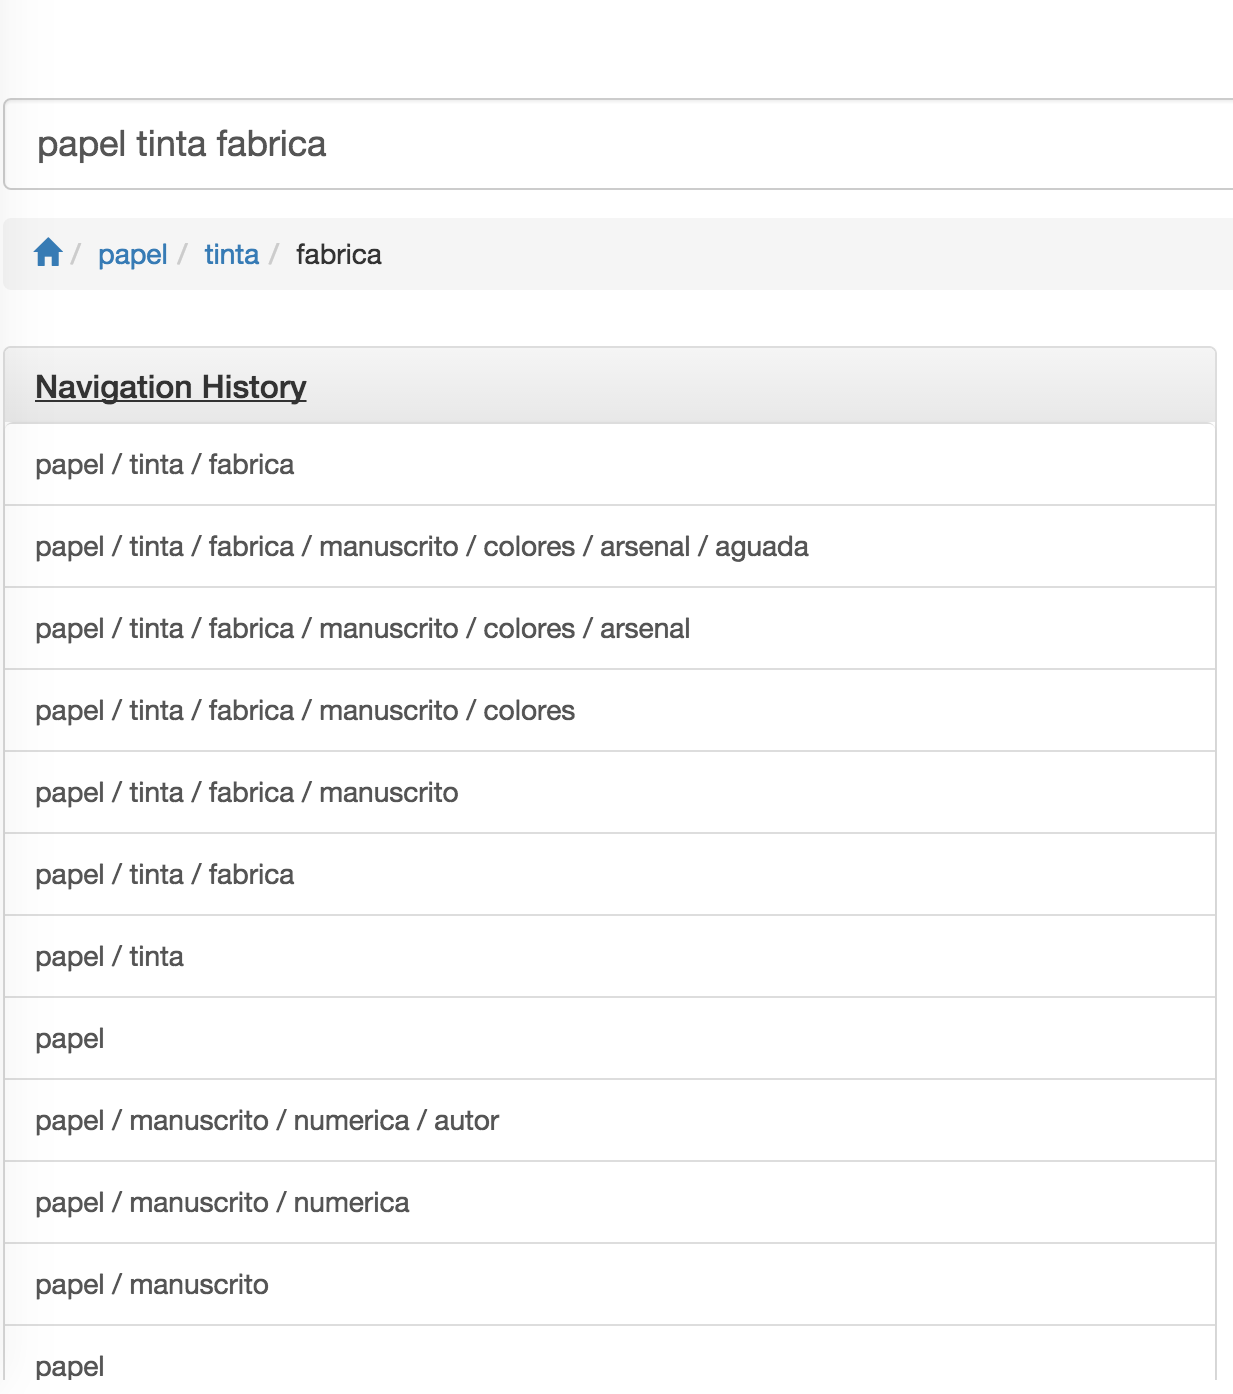
\includegraphics[width=.48\linewidth]{images/fancy3}
\caption{Fancy FCA 1.0, the Focus is ``papel tinta fabrica''. In the left picture, you can see the Results. In the right picture, you can see the Navigational History.}
\label{figure:fancy3}
\end{figure}

When the user starts browsing, a \GLS{JSON} file with all the data is downloaded to his client. The file contains the information of the lattice and also about the documents. The programming logic is done on the client side. This reduces the communication between the client and the server to a minimum because all the data is already at the client. It just has to be decided which parts of the data are shown to the user. For instance it 

\section{Discussion}
\label{fancydis}

For the concept, it is to question if the bubble cloud is an appropriate technique to show the Suggestions. The Suggestion consists of terms and a number of documents. This information can also be shown in a table. A table is structured to present information. But the bubble cloud avoids a clear order in the data. In a table, probably only the top suggestions would be considered. This is dangerous, because the number of documents a suggestions represents should not guide the users. What is also to question, is that only children of the Focus are currently presented. For now, the parent formal concepts of the Focus are ignored. In the next iteration of this software, it would be useful to make use of the parents as well.\\

The implementation has a problem because of the huge size of the \GLS{JSON} file. The user has to download over eight megabytes before she can start using the interface. The user also needs a computer with a lot of memory because the browser has to handle a lot of data. In this case, the eight megabytes are compressed and the browser uncompresses the data to over 80 megabytes. Especially older computers may have problems with this webpage. The design decision to download all the data upfront was made before it was clear that the \GLS{JSON} file would be so huge. This can be fixed by porting the programming logic from the client side into the server side. By doing this, only the data that is currently needed would be send to the client. This would require more communication between client and server but greatly reduces the amount of data that the browser has to handle. \\

 It would also be a good idea to include thumbnails of the the maps to the result. This could not be done, because it was not possible to get thumbnails of the maps. This should be fixed in further iterations of the software. It was also decided to show only the 100 first results in the result list because of browser performance reasons. To fix this, it should be allowed to reload additional results.

\chapter{Evaluation}
\label{Evaluation}

The design of an interface is highly subjective. User studies can help to evaluate the quality of an interface. For this, a brief review of different techniques for human studies is given first. Then I describe the setup of the study, followed by the results and finally conclusions.

\section{Background}

We will only scratch the surface here. A comprehensive introduction into "Methods for Evaluating Interactive Information Retrieval Systems with Users" gives Kelly \cite{Kelly2007}. A shorter introduction suited for "User Search Interfaces" gives Hearst in Chapter 2 of her book \cite{Hearst2009}.

\subsection{Basics}

So we want to measure quality of an interface which is its usability. How is usability defined? The ISO 9241-11, 1998 \cite{ISO} defines three aspects of usability:
\begin{itemize}
	\item Effectiveness: Accuracy and completeness with which users achieve specified goals.
	\item Efficiency: Resources expended in relation to the accuracy and completeness with which users achieve goals.
	\item Satisfaction: Freedom from discomfort, and positive attitudes towards the use of the product.
\end{itemize}

\subsection{Experiment vs. Evaluation}

It is important to distinguish between the terms ``experiment'' and an ``evaluation''. Kelly \cite{Kelly2007} writes:
\begin{quote}
Evaluations are conducted to assess the goodness of a system, interface or interaction technique and can take many forms [..] Experiments have historically been the main method for interactive system evaluation, but experiments can also be conducted to understand behavior [..] Two important characteristics of experiments are that there are at least two things being compared (e.g., system type) and that some manipulation takes place [..] In some types of [interactive information retrieval studies] only a single system is evaluated. This is a weaker form of evaluation since it is not possible to demonstrate how much better users perform or how different their behaviors and inter actions are since there is no point of comparison. Traditional usability tests are examples of this type of evaluation. Traditional usability tests are usually conducted with a single version of a system, with the goal of identifying potential usability problems.	
\end{quote}

In this thesis, the system is only evaluated to find usability problems. No comparisons among other systems are conducted but should be done in further investigations.

\subsection{Informal Usability Testing}

Hearst \cite{Hearst2009} describes Informal Usability Testing as "Showing designs to participants and recording their responses". It is often used in short iterative cycles to quickly evaluate a design. In this thesis, only informal usability studies are conducted because the conductors do not have proper equipment nor any experience with other user studies.

\subsection{Questionnaires}

A questionnaire comprises a set of questions and is a cheap and fast way to gather information from people. Kelly et al. \cite{Kelly2008} describe two types of questions as follows:

\begin{quote}
	Questionnaires can be comprised of closed questions, open questions or a mixture of both. \textit{Closed questions} are questions that provide a fixed set of responses with which subjects must respond. It is common practice for usability questionnaires to include closed questions in the form of statements such as, the system was easy to learn to use. Subjects are typically provided with 5–7-point Likert-type scales for responding, where one scale end-point represents strong agreement and the other represents strong disagreement. [..] \textit{Open questions}, on the other hand, do not provide a response set and subjects are able to provide any type of response they feel is appropriate. 
	\end{quote}


\subsection{Thinking Aloud}

Kelly \cite{Kelly2007} explains by referring to Ericsson and Simon \cite{Ericsson1993} that the think-aloud method asks subjects to articulate their thinking and decision-making as they engage with the interface. The comments from the participants have to be collected. Either by recording the evaluation session or by taking notes. It is hoped that the conductors can learn from the thinking process of the participant. There exist variations of this technique. Because it can be exhausting, challenging and awkward to talk to yourself all the time, participants are encouraged to report either at some fixed times or when they want.

\section{Setup}

Sadly, I only had minor influence on the setup of this study because I was not allowed to set it up. The conductors in charge where amateurs and did not have any experience with human studies. The evaluation was done with five people with a background in humanities. The demographic background was only collected from three participants: Female 60 years old, female 49 years old, male 44 years old. All participant listened to an introductory presentation which was given in Spanish. I do not know what was the content of the presentation because I do not understand Spanish well enough. The participants were split into two groups: One with three participants and one with two participants. These two groups sat in the same room approximately four meters away from each other. They were split into groups because there was not enough time to do individual evaluation sessions.\footnote{Not my decision.} All members of a group sat in front of \textit{one} computer. The participants rotated in front of the computer\footnote{Not my decision.}. I was responsible for the group with three participants. From the group with two people, it was not possible collect data during the session. All five participants filled out a questionnaire after the session. So now I will just describe the procedure of my group. \\

	After the introductory lecture, all participants got a handout. The handout consists of four parts:
\begin{enumerate}
	\item A description of the interface. But this was an academic text and not meant to be a manual. I doubt that anybody read it.
	\item Four Tasks the participants should do. They are included in the Appendix~\ref{app:tasks}. I do not think that these tasks were suited for a user study. They were too long and they revealed to much to the user. In my opinion, the user has to figure out on her own how to solve a given task. The third task was not even doable.
	\item A questionnaire with ten\footnote{Chosen by me.} closed questions from USE questionnaire \cite{lund2001measuring}. The question are also in the Appendix~\ref{app:closed}.
	\item Three\footnote{Chosen by me.} open questions as asked by Kelly \cite{Kelly2008} and additionally one question which should compare the evaluated system with the original search engine\footnote{\url{http://www.mcu.es/ccbae/es/consulta/resultados_busqueda.cmd?busq_codsecc=MCAGS}}. It was not my idea to include this question. It is out of the scope of the study setup and it was not planned to show users the other search engines. All four questions are in the Appendix~\ref{app:open}.
\end{enumerate}

During the session, I encouraged the participants to talk to me while they were using the interface. I did not force them to speak to me all the time, but I asked them from time to time. The session was recorded with an iPhone 6 Plus\footnote{\url{https://www.apple.com/iphone-6}} and analyzed afterwards. The instructor wanted the participants to do the tasks, but I knew that the tasks were nonsense and persuaded the participants to just use the interface. But after some time, I had no excuse left not do the tasks so I gave in and let them do the tasks. At this time, I already collected enough data. After approximately  55 mins the session was done and the participants filled out the pen-and-paper questionnaires - in Spanish. The instructor allowed the participants to fill out the questionnaire in Spanish. This made the analyzes of the open questions very difficult. Even though they were translated, I did not have access to all information of the written responses because the translation process was not carefully done.
\section{Results}

It was hard to extract knowledge from this chaotic study setup. I divided the results into two categories: closed questions and everything else as \textit{comments} to keep things short. There were not any major differences between the verbal comments during the session and the responses to the open questions. This can also be due to the fact that I did not have access to the original sources and only to a flawed translation. It is also worth mentioning that the evaluation study was the first time for the participants to use a FCA-based system. This lead to some comments on the approach itself.

\subsection{Comments}
All participants wrote down and said they were missing the possibility to refine the search by a time range, location and author. They said that this is very important for their work. In addition, one participant could not believe why the search was not working when she searched for ``Valencia''. The term was not included in the word list and thereby not in the lattice. So the search resulted in an empty search result. She mentioned that this should get fixed immediately. One participant said that she thinks the content of the concept lattice is biased. She thinks other terms would be better. Another participant disagrees and thinks that the words are appropriate. \\

I confronted one participant with the question what exactly they need, because I think that the original search engine\footnote{\url{http://www.mcu.es/ccbae/es/consulta/resultados_busqueda.cmd?busq_codsecc=MCAGS}} already offers what they are asking for. She responded that she thinks I am right. But she also showed the search engine sometimes fails to deliver results\footnote{It was not clear what exactly was the problem with the search engine}. In addition, I showed her another website which displayed old maps: \url{http://www.oldmapsonline.org} \footnote{Screenshot in Appendix~\ref{app:oldmaps}}. She responded that she liked the idea. \\

Two participants gave suggestions to improve the result list. Both said that the thumbnails should definitely be included and that they were not interested in the text snippet of the result. The text snipped showed part of the annotations of the resulting map. By removing the text snippets and thereby reducing the height of a result item, they could see more results at once. They were very interested to see the titles of the results. No participant used the possibility to save documents. Two participants said they thought it a good idea to link to the original website. One participant explained that she is very interested to see related maps to a given map. This would be the original way how humanists do their research. It is my fault that this function was not included in the system. \\

In regard to the appearance of the interface in general, the comments were positive. The participants liked the clean design. One participant wrote that using the system was funny. Two participants said they liked the interface but not the content. Two participants wrote, it is easy to use. I observed that the users did not use the search very often. They were more interested in the skimming over the bubble cloud.

\subsection{Closed Questions}

\begin{table}[h]
\caption{Responses from closed questions. Participants (n=3) had to choose between 1 (disagree) and 7 (agree). }
\label{table:closed}
\centering

\def\arraystretch{1.2}% 
\begin{tabular}{ | l | c |}
\hline
& Average Response\\
\hline
\large{Usefulness}&\\
It is useful.&$6.\bar{6}$\\
It meets my needs.&$4.\bar{3}$\\
It does everything I would expect it to do.&$4.\bar{3}$\\
&\\
\large{Ease of Use}&\\
It is easy to use.&$7$\\
It requires the fewest steps possible to&$5.\bar{6}$\\
accomplish what I want to do with it.&\\
I don't notice any inconsistencies as I use it.&$5$\\
&\\
\large{Ease of Learning}&\\
I learned to use it quickly.&$6.\bar{6}$\\
I easily remember how to use it.&$6.\bar{6}$\\
&\\
\large{Satisfaction}&\\
I am satisfied with it.&$5.\bar{6}$\\
It is fun to use&$5.\bar{6}$\\

\hline

\end{tabular}
\end{table}

Out of the five participants only three filled out the questionnaire. All results are in the Appendix~\ref{app:closed}. The average responses are shown in Table~\ref{table:closed}. The results correspond to the comments made by participants. The weakest results got the sentences "It meets my needs" and "It does everything I would expect it to do". This also makes clear that the participants did not like the content of the interface. The best result got the sentence "It is easy to use". Overall the results are positive, but it is hard to draw conclusions because it is not clear how the bad content affected the perception of the user. The study should be repeated in a case when the concept lattice itself is useful. This would yield better results.

\section{Accessibility Analysis}

In addition to the evaluation session, there was an evaluation regarding accessibility\footnote{If people with disabilities can use the interface.}. It was conducted by people from the UNED: Miguel Angel Marqueta and Covadonga Rodrigo San Juan. The report can be found in Appendix~\ref{app:access} but they also did some verbal comments which will be told here. Their comments were overall positive but they highlighted some problems with the interface: It is possible to zoom in the bubble cloud, but there are no buttons on the screen for it. In the current state, the zooming can only be done with a mouse or a touchpad. They also pointed out that the users cannot see if the result list was updated. The users should get more feedback when the result list updates after a navigation change. They mentioned that the heart icon to bookmark documents may be misleading and should be changed. 

\section{Conclusions} 
Zobel \cite{Zobel2004} proclaims that far too many human studies in computer science are amateurish and invalid. I have to admit that this study is one of those amateurish studies. In addition to the chaotic setup, it is hard to draw conclusions because of the low number of participants. But it can be said that the way FCA was applied to the documents collection does not suit the needs of the users. It is very confusing for the users that they cannot search for arbitrary terms on the lattice. It is also a major problem that the users cannot refine their information needs along dimension. They want to specify exact time ranges, locations and authors. FCA cannot offer this because it only works on one-dimensional data. For the future, techniques like faceted search as described in Section~\ref{dyafs} and/or interfaces like \url{http://www.oldmapsonline.org/} \footnote{Screenshot in Appendix~\ref{app:oldmaps}} should be applied.\\
 
For the interface itself, it looks like the users found it easy to use and easy to learn it. But there are problems with the presentation of the result list. But also other minor problems were found. These problems should be addressed in future iterations of the software. It is to question, if the users want to bookmarks search results. The results always link to a web page. So it can be argued that it is not necessary to offer this possibility. The users can just bookmark in their own browsers.

\chapter{Fancy FCA 2.0}
\label{Fancy 2.0}

The evaluation clearly showed that an FCA-based approach does not fulfill the needs of its potential users. But as we talked about in previous sections, it is used in other areas. That is why the work that resulted from the thesis could be useful to visualize arbitrary concept lattices. I decided to transform Fancy FCA 1.0 into a general tool to visualize concept lattices. Besides all the improvements I suggested in the previous suggestions (make use of the parents of the Focus, improve result list), there are some major changes. This section is a mixture about changes that were already made and an outlook that still needs to be done, it is still work in progress. This is the second version of my work and therefore it is called Fancy FCA 2.0. It will be available on the web: \url{http://fca.vis.one}.\\

To simplify the tool, some functionality was dropped: All logging is removed. In addition, the whole user authentication is removed as well. This means that it is not possible to bookmark documents. Also the history is only saved for the current \gls{session}. This was done because it looks like the user did not find this very interesting.\\

What has to be included: Users should have the possibility to upload concept lattices. For the sake of simplicity, they can do it anonymously without any authentication. This also means that in this first version of this tool, already uploaded data cannot easily be removed. As discussed in Section~\ref{fancydis}, Fancy FCA 1.0 has a design flaw: The complete data has to be loaded to the browser upfront, when someone uses the website. This is especially harmful because this tool should address large lattices and large lattices can be very big. To address this, most of the program logic is done on the server side. This means that the client only gets the data of the current Focus. When she changes the Focus, the browser sends a request to the server to get the new data. The data on the server has to be stored efficiently. I use mongodb\footnote{\url{https://www.mongodb.org/}} for that because it is easy to store hierarchical data in it. The MySQL databases is not needed anymore. \\

The implementation of this changes is not finished yet and can be followed here: \url{https://github.com/filter1/fancy}.

\chapter{Conclusions}
\label{Conclusions}

First, as described in the introduction, digital humanities is the intersection between humanities and information technologies. This boils down to the development of digital tools for human scholars. This was also the underlying task the research group should do, but: Building tools is NOT the primary focus of computer science research. Computer science research is mainly focused on finding new algorithms, refining algorithms, applying algorithms to new problems etc.. Computer scientists are not famous for being the best software engineers. It is a very bad idea to take computer scientists and say to them: ``Now build some tools for human scholars!'' as this was done in this case. As this thesis showed, this approach was quite a failure. The researchers wanted to apply bleeding-edge methods, like FCA, when building these tools. But all the human scholars (supposedly\footnote{Requirements were never defined.}) needed, was a very simple search interface with some custom query filters. But at least for an ordinary computer scientist, this is not very challenging and so they are trying some sophisticated methods. To do real research in digital humanities, people are needed who live and breathe digital humanities. I think, this is the reason why wise people coined the term ``digital humanities'' to make clear that it is fundamentally different from computer science research. \\

Second, I proposed a method to visualize large concept lattice. It focuses only on small parts of the lattices and the user can incrementally explore the lattice. Thereby she feels confident to explore the lattice because she can always backtrack to earlier actions. I can say with slight confidence\footnote{The evaluation setup was very chaotic.} that the users liked this approach. But further user studies are needed to judge if my proposal suits the needs of the users. \\

Third, for the use of FCA in information retrieval, the evaluation showed that it is difficult. If the concept lattice is build from a word list of possible index terms, it can irritate the users why only a small portion of all possible words is in the concept lattice. This procedure does not look promising and should be avoided in future research.
\newpage
\bibliographystyle{plain}
\bibliography{biblography}

\newpage
\appendix
\chapter{Appendix: Accessibility Report}
\label{app:access}

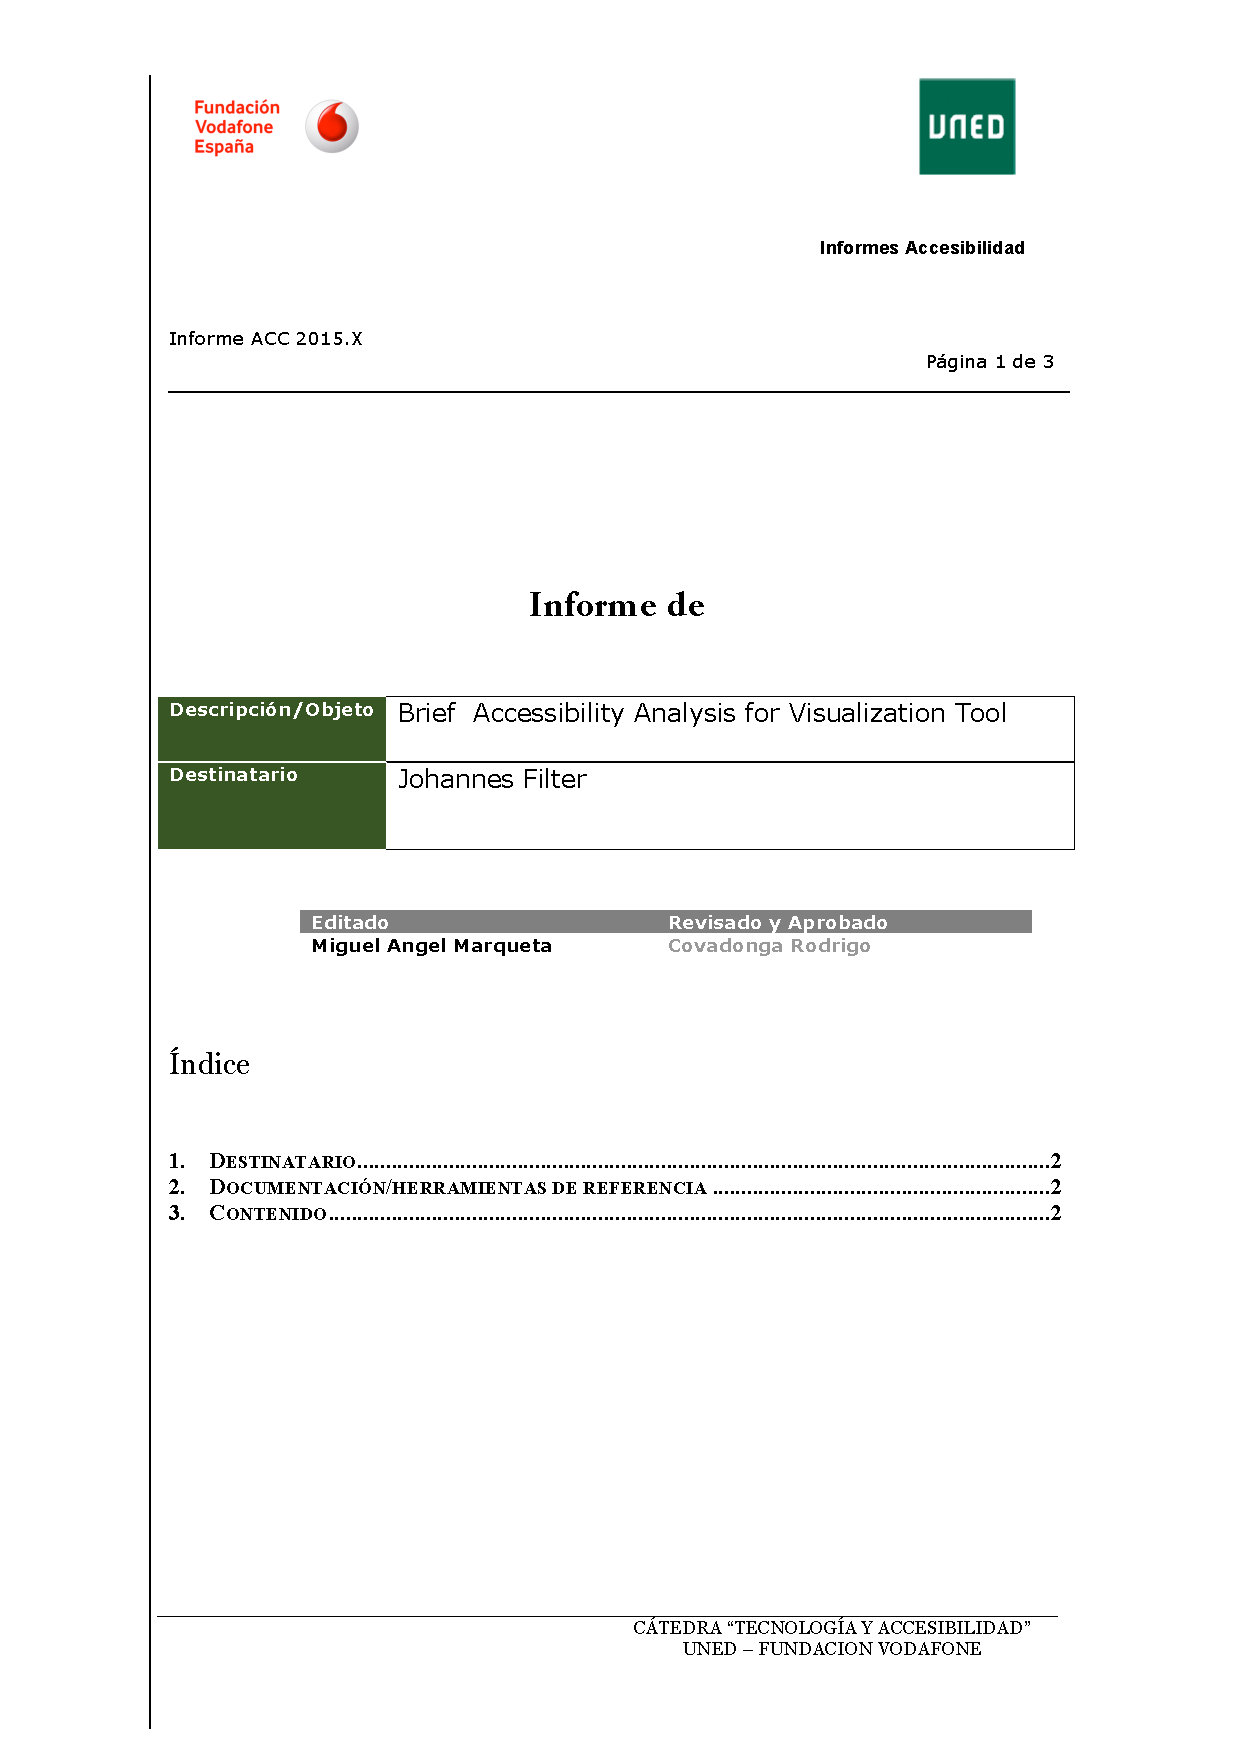
\includepdf[pages={-}]{appendix/report.pdf}

\chapter{Appendix: Closed Questions}
\label{app:closed}

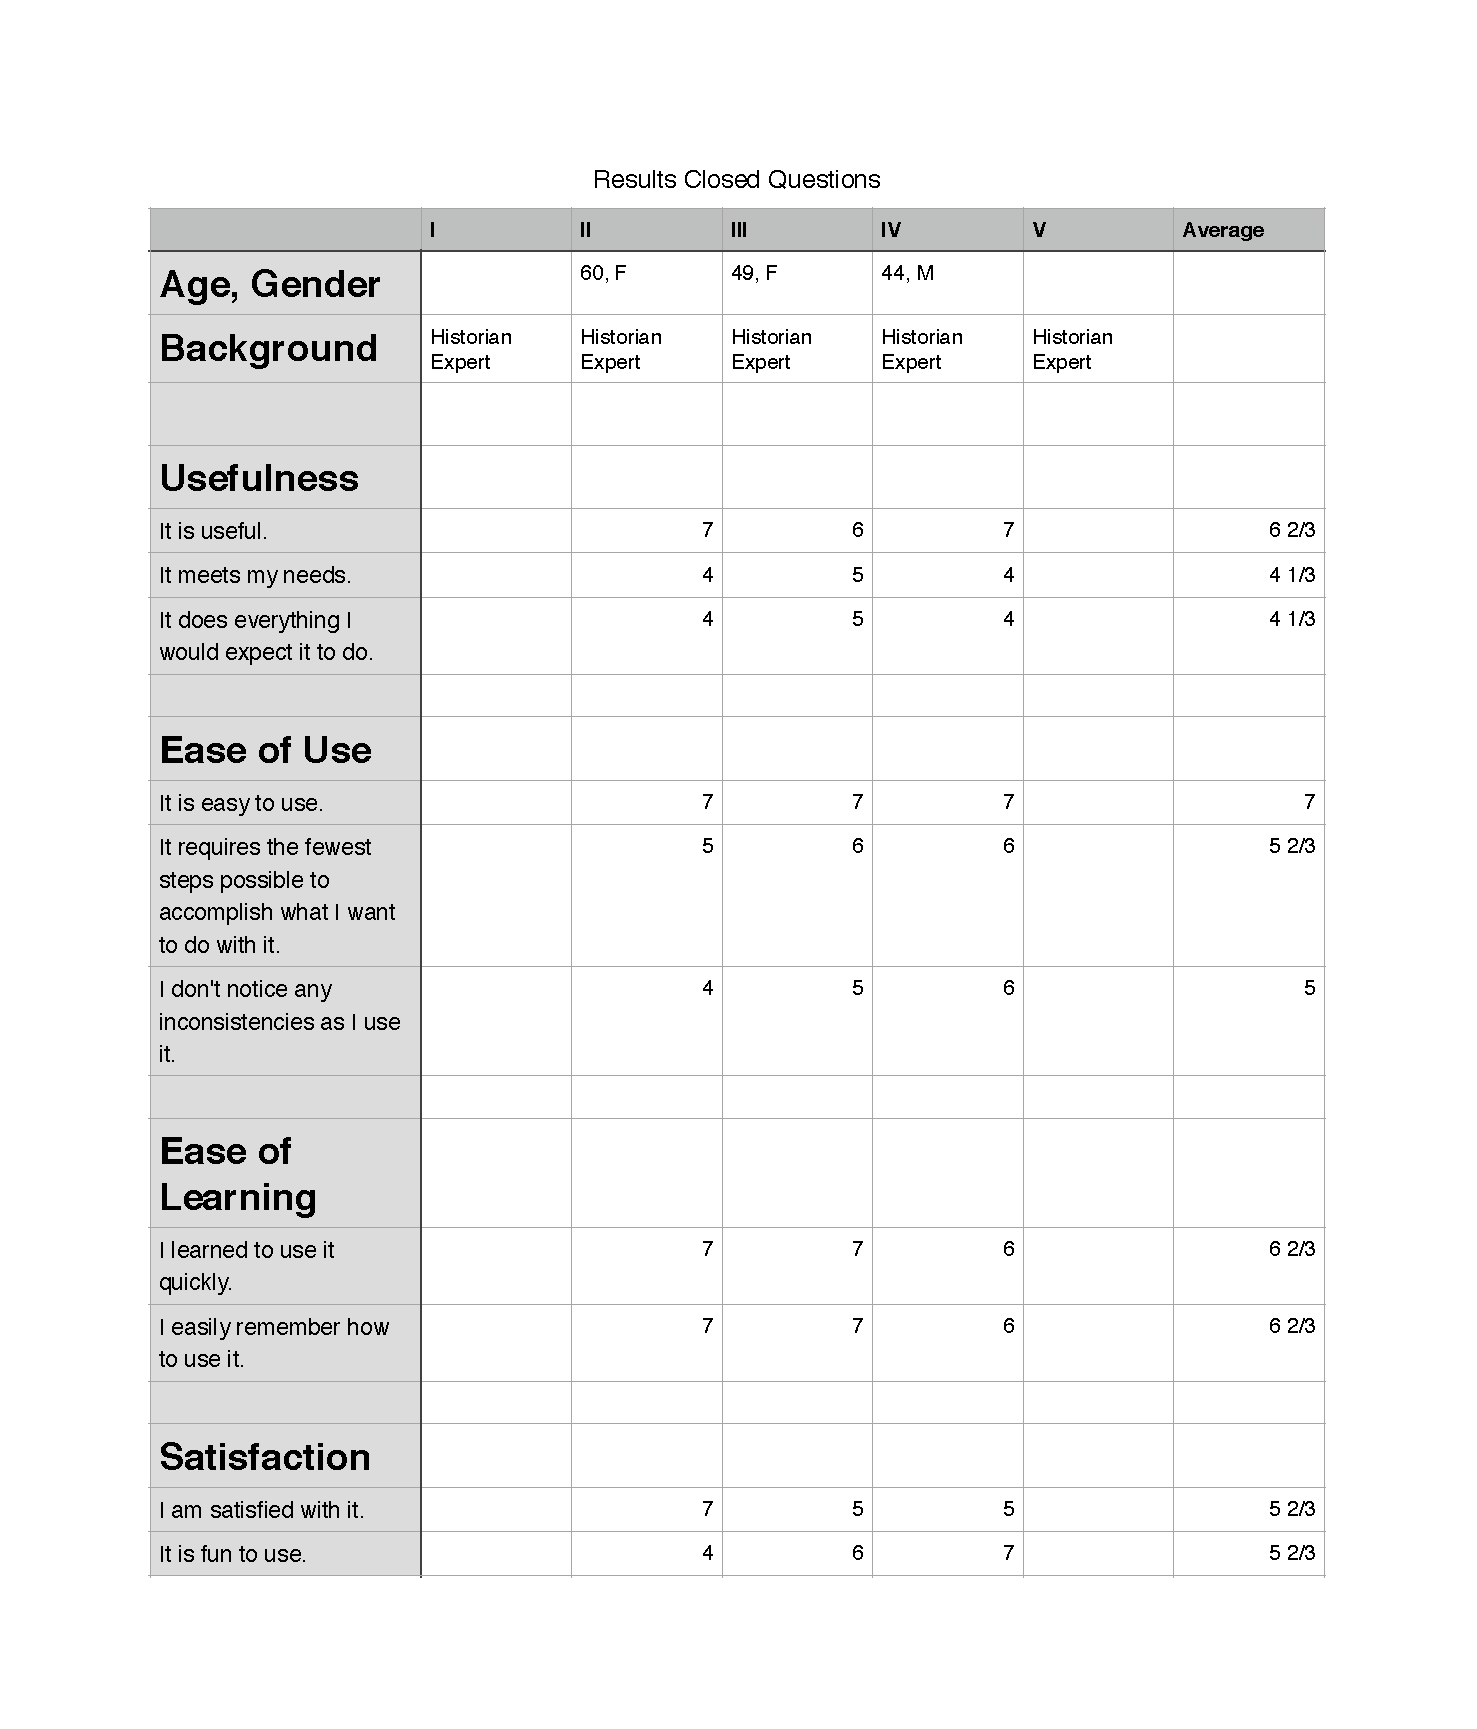
\includepdf[pages={-}]{appendix/closed.pdf}

\chapter{Appendix: Open Questions}
\label{app:open}

\begin{itemize}
	\item What were the most positive things about using this system and why?
	\item What were the most negative things about using this system and why?
	\item How would you improve this system and why?
	\item Is there anything else that you would like to tell us about this system and your experiences using it?
	\item In comparison with other systems (Interface of Catálogo Colectivo de las colecciones de Mapas and previous work of this research group).
Do you think it is more useful? If yes, which part of the system is more useful.
\end{itemize}

\chapter{Appendix: Tasks}
\label{app:tasks}
\begin{enumerate}
	\item The user is not looking for a particular topic. He/she starts with the general empty overview of the topic. He/she picks a word from the bubble cloud and navigates to new concepts. He/she repeats this procedure for several times. He/she is using the breadcrumbs to go up again and looks for some other words. He/she finally finds one interesting item and studies it on the original AGS website.
	\item The user wants to find information about one term (``mapa'') that interests him. Before he/she starts browsing, he/she logs into his user account. After that, he/she typed in the search interface the term and makes use of the type-ahead. He/she finally gets to the desired concept and reviews the concepts. He/she decides to get more specific ones and refines the search by clicking on words in the cloud. He/she finds interesting documents and bookmarks them for later investigations. He/she goes back again by using the breadcrumbs and chooses another term. He/she finds other interesting items and bookmarks them.
	\item A humanist expert is working in the DIMH project. He/she has an extensive knowledge about the historical scenario related to the project: the engineers in the service of the Spanish Monarchy in the XVI and XVII centuries. He/she is trying to draw some conclusions about the work conducted by these engineers and also about the different aspects related to their works (e.g., typology of their projects, technical details about their way to work, relationships between them and the monarchy, preferred locations for their projects...). To that end, he/she makes use of the AGS collection, which includes an extensive catalogue of draws, maps and plans about different projects conducted by those engineers.
He/she is used to manually analyze this kind of collections; however, the size of the AGS dataset (almost 8000 files) makes the manual analysis difficult. Therefore, he/she takes advantage of the visualization tool showing the dataset modeling and organization to analyze its information.
In particular, he/she is interested in the analysis of the projects carried out by Jose Patino. The user is aware that Jose Patino carried out some projects in the city of Sevilla, and he/she wants to have more information about these projects as well as to find some other projects with similar characteristics in other cities
	\item The same humanist expert is now looking for information about projects made in the coast (e.g., fortifications in the coast). He/she knows that the engineers used different metrics (e.g., pies-reales, varas) to measure the distances. Moreover, he/she believes that it could be some relation between these metrics and the date of the projects. More in particular, he/she believes that ``varas'' was not used before the XVII century, while ``pies-reales'' was a common metric, even in the XVI century.
Furthermore, he/she wants to explore if there is also another aspects (i.e., beside the temporal issue) related to each one this metrics.
\end{enumerate}

\chapter{Appendix: oldmaps}
\label{app:oldmaps}

\begin{figure*}[!ht]
	\centering
	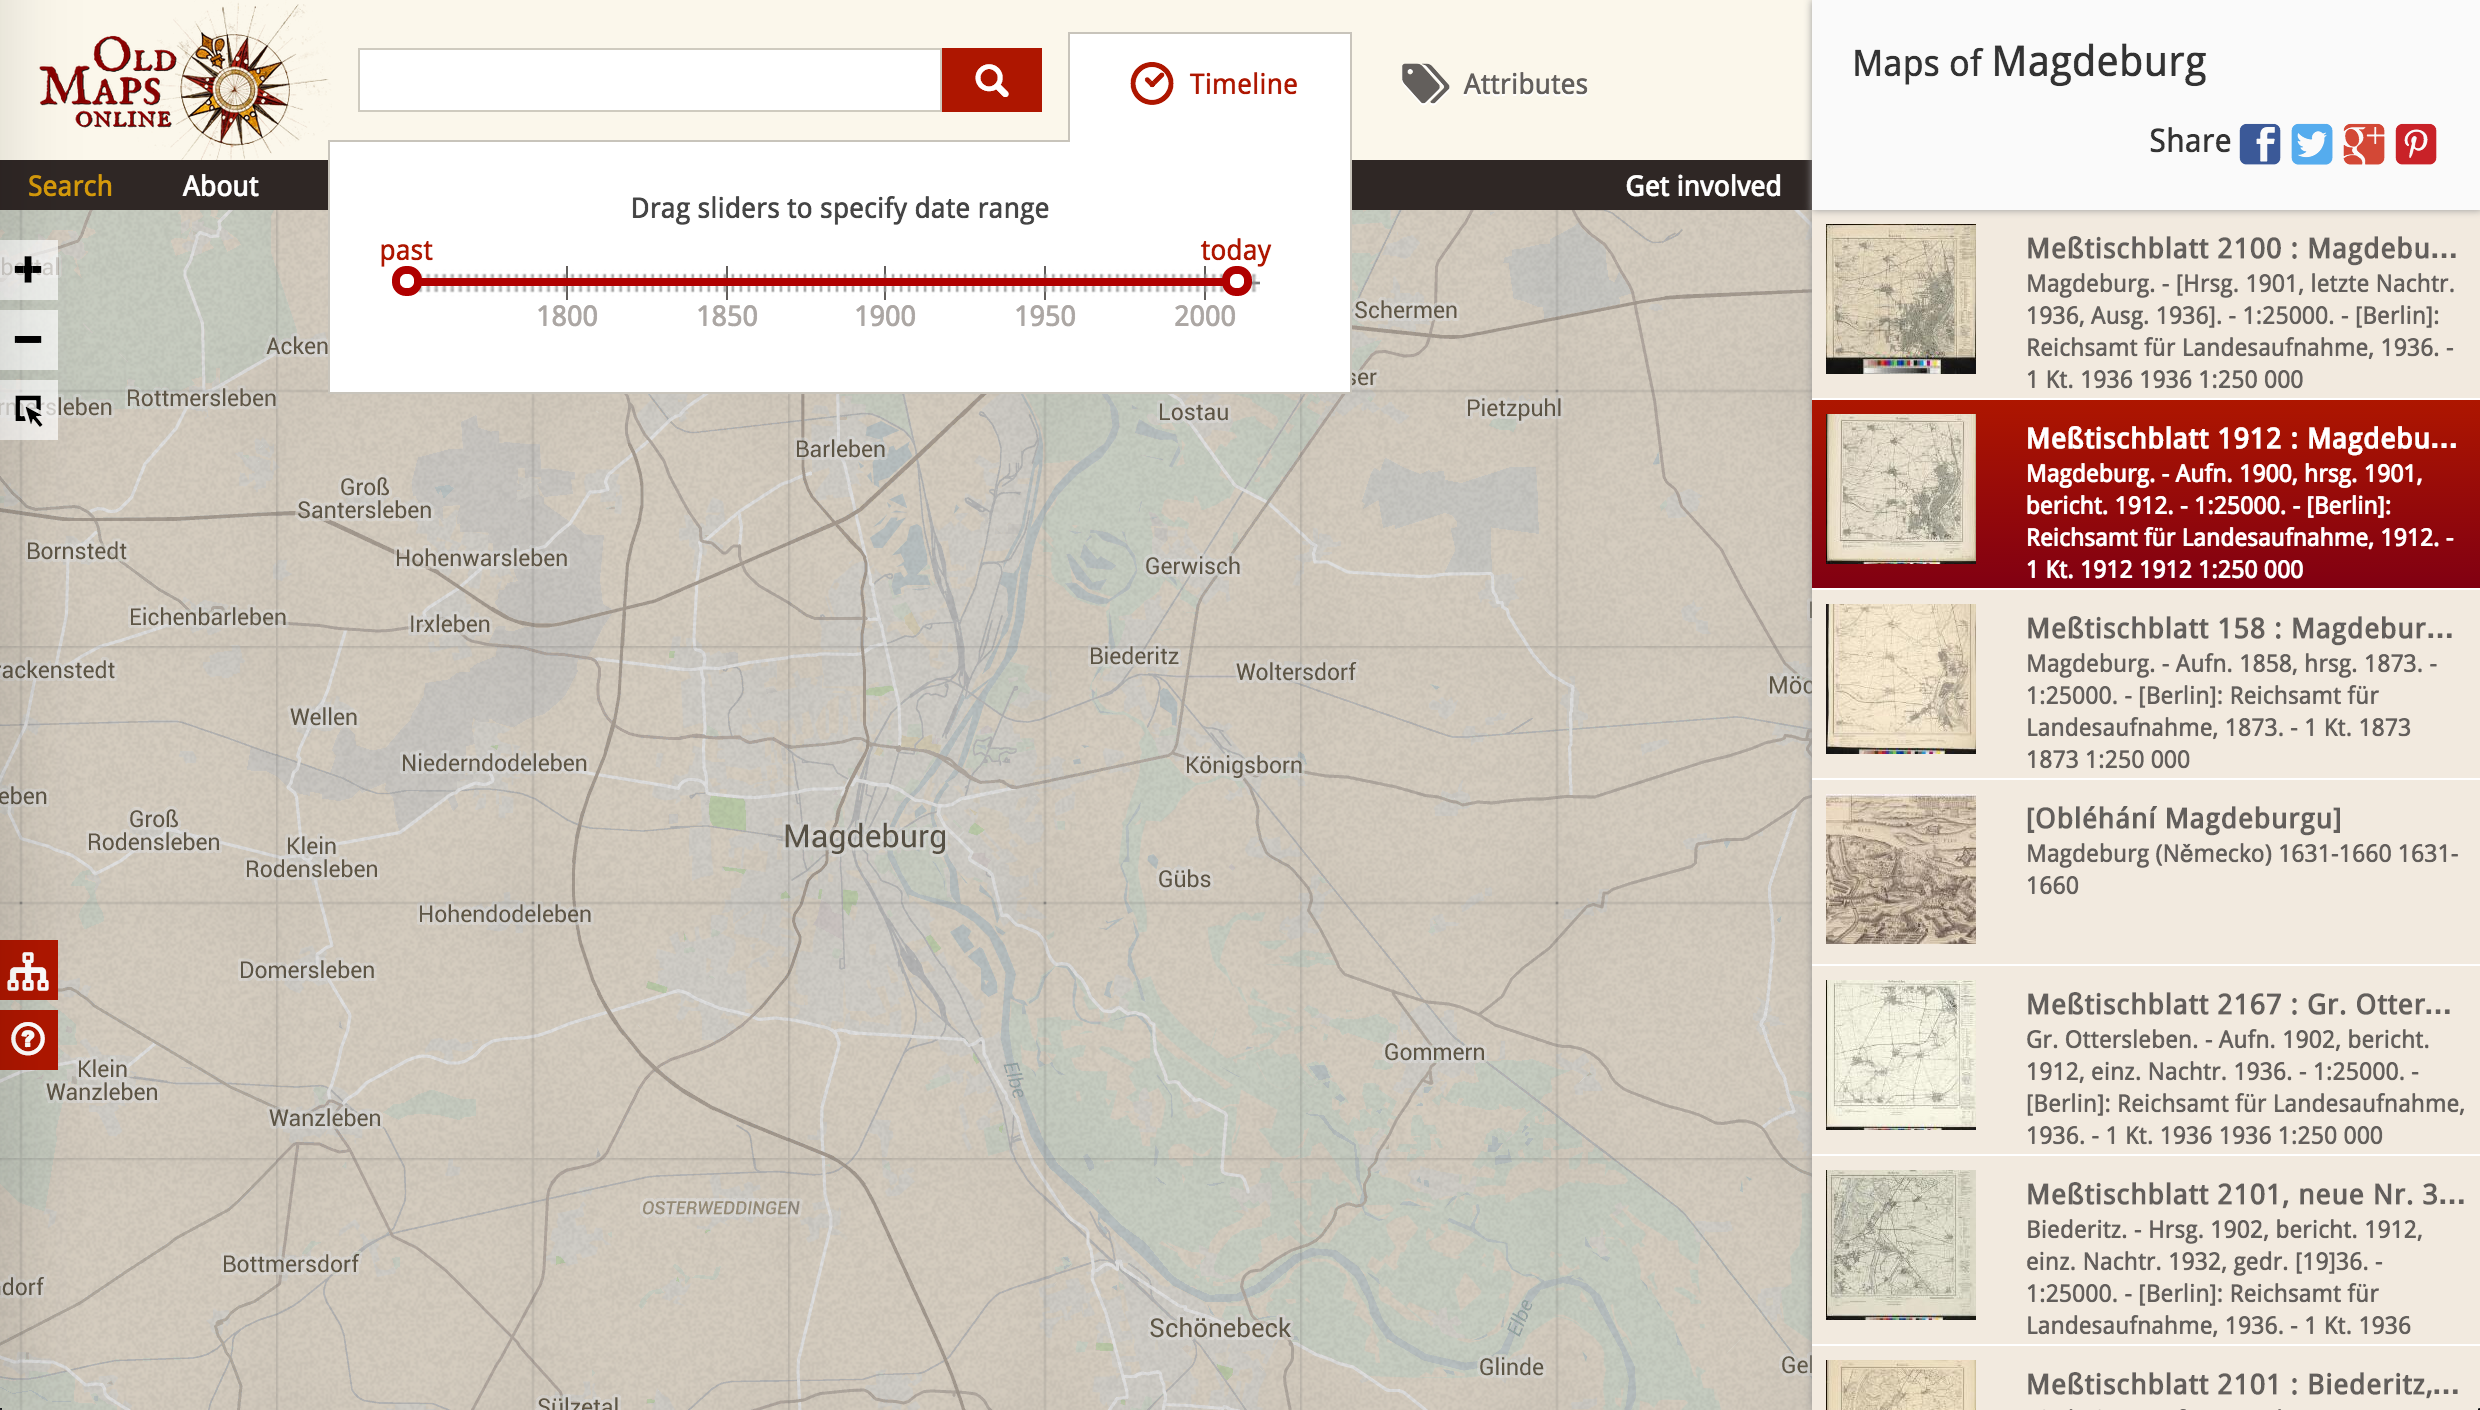
\includegraphics[width=\linewidth]{images/oldmaps}
\caption{Screenshot of \url{http://www.oldmapsonline.org/} with focus on Magdeburg. Users can specify time ranges.}
\label{figure:oldmaps}
\end{figure*}


\newpage

\chapter*{Eigenständigkeitserklärung}

Ich versichere hiermit, die vorliegende Arbeit selbst verfasst, Zitate gekennzeichnet und keine anderen als die offengelegten Quellen und Hilfsmittel benutzt zu haben.\\



\end{document}